\subsection{General results of the framework}
\subsubsection{Movement and Diffusion}
The movement of the microbial agents showed the random dispersal of the microbes over the grid environment (Figure \hyperref[fig:mov]{\ref{fig:mov}}). The same was also observed in the diffusion model, where the metabolite flowed to the lowest concentrations on the grid (Figure \hyperref[fig:diff]{\ref{fig:diff}}).

\begin{figure}[h!]
  \centering
  \begin{minipage}[t]{0.3\textwidth}
    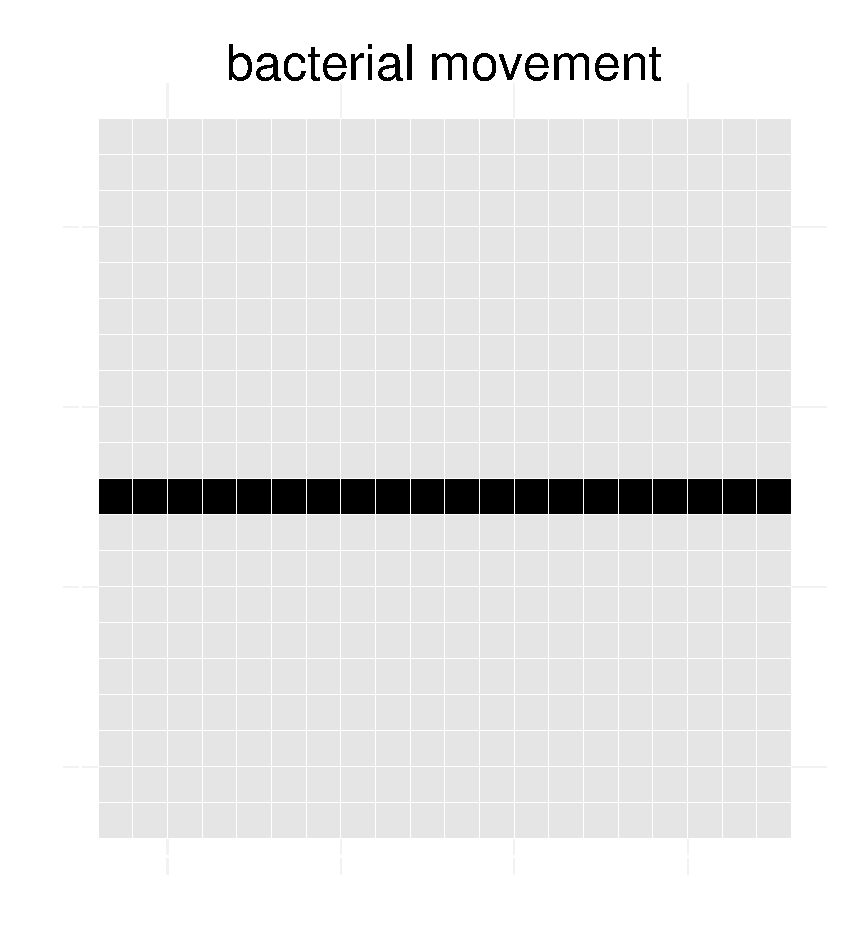
\includegraphics[width=\textwidth]{mov1.pdf}
  \end{minipage}
  \begin{minipage}[t]{0.3\textwidth}
    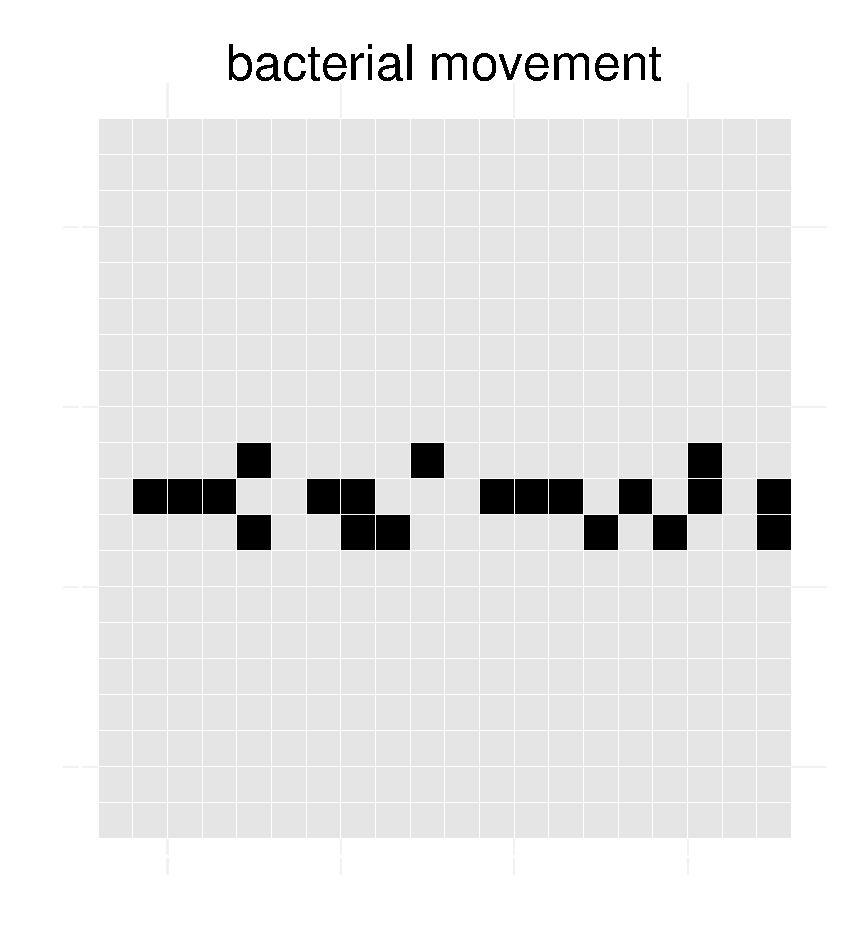
\includegraphics[width=\textwidth]{mov2.pdf}
  \end{minipage}
  \begin{minipage}[t]{0.3\textwidth}
    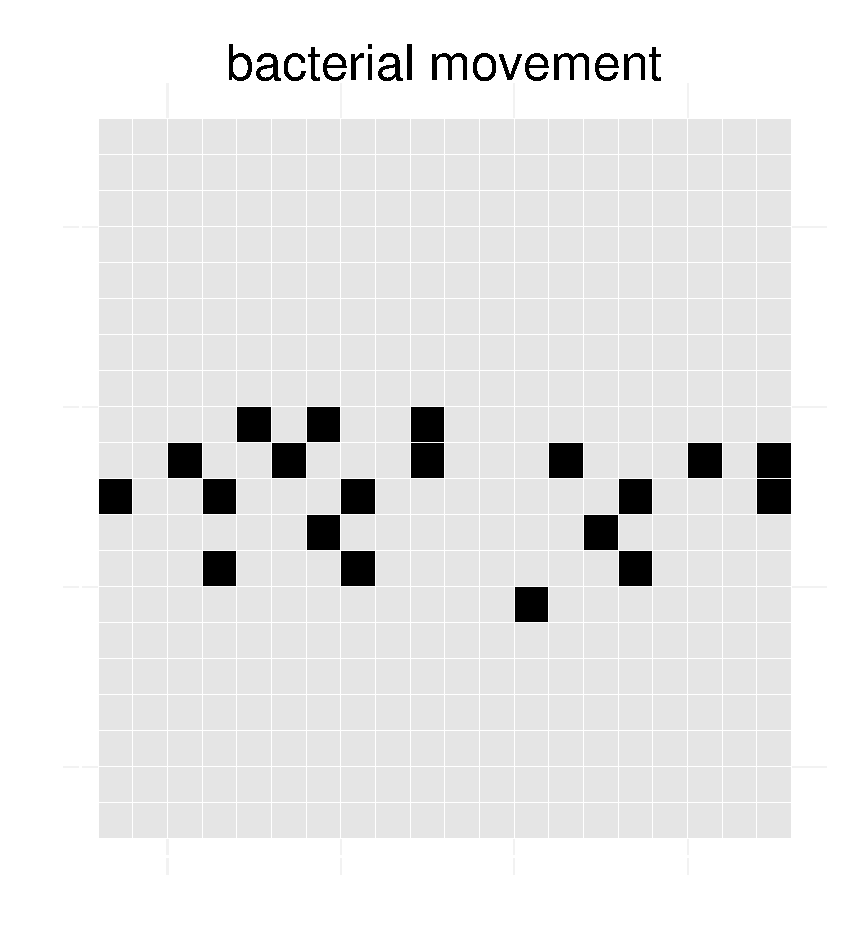
\includegraphics[width=\textwidth]{mov3.pdf}
  \end{minipage}
  \caption{Bacterial movement starting with a line of bacteria in the middle of a $20\times20$ grid. Three different iteration steps are displayed (time step 1, 2 and 5).}
  \label{fig:mov}
\end{figure}
\begin{figure}[h!]
  \centering
  \begin{minipage}[t]{0.3\textwidth}
    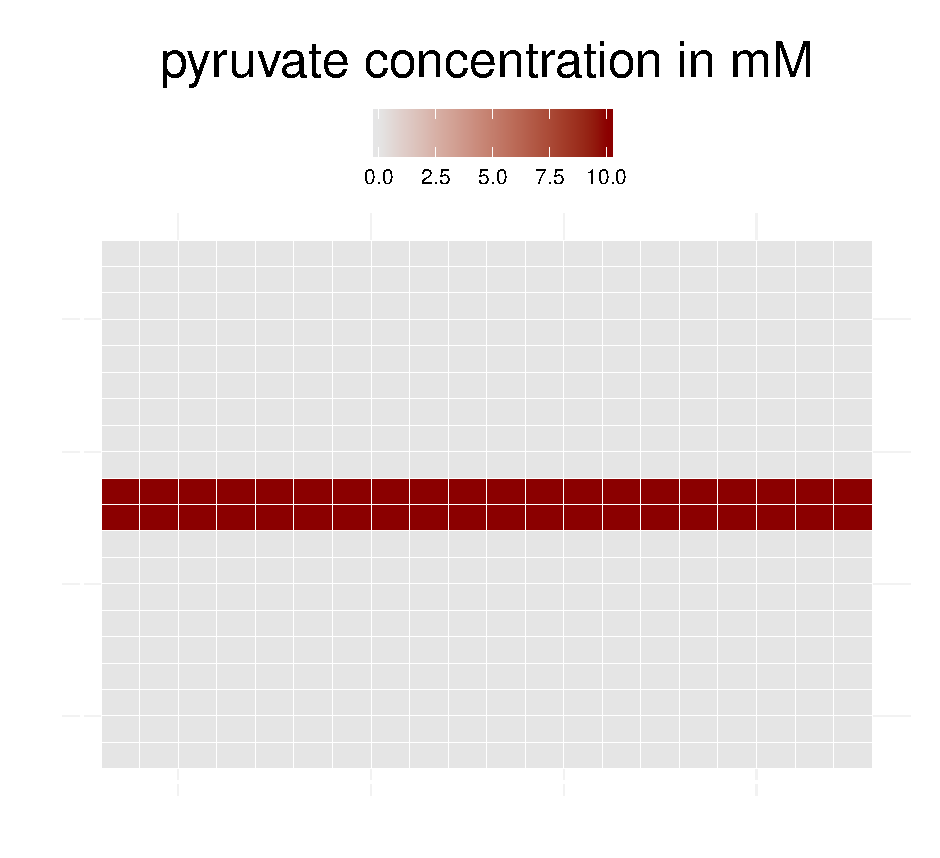
\includegraphics[width=\textwidth]{diff1.pdf}
  \end{minipage}
  \begin{minipage}[t]{0.3\textwidth}
    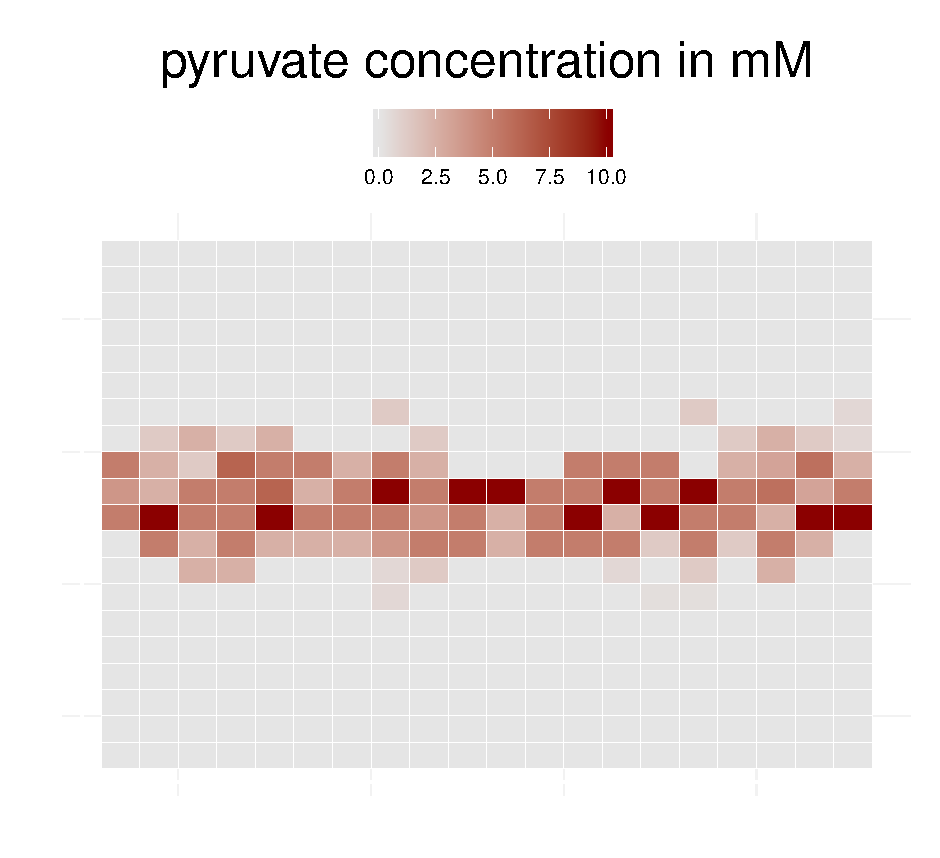
\includegraphics[width=\textwidth]{diff2.pdf}
  \end{minipage}
  \begin{minipage}[t]{0.3\textwidth}
    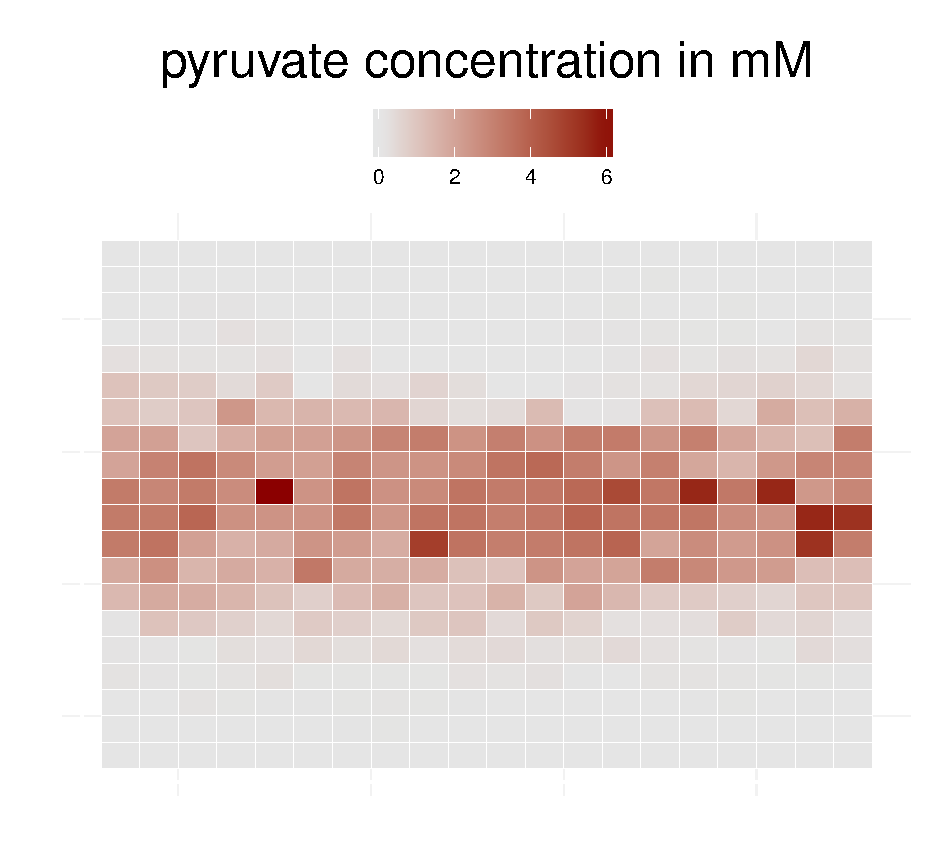
\includegraphics[width=\textwidth]{diff5.pdf}
  \end{minipage}
  \caption{Diffusion starting with 10\;mmol pyruvate in the middle of a $20\times20$ grid. Three different iteration steps are displayed (time step 1, 2 and 5).}
  \label{fig:diff}
\end{figure}

\subsubsection{Time consumption}

\begin{figure}[h!]
  \centering
  \subfigure[]{
  \begin{minipage}[t]{0.45\textwidth}
    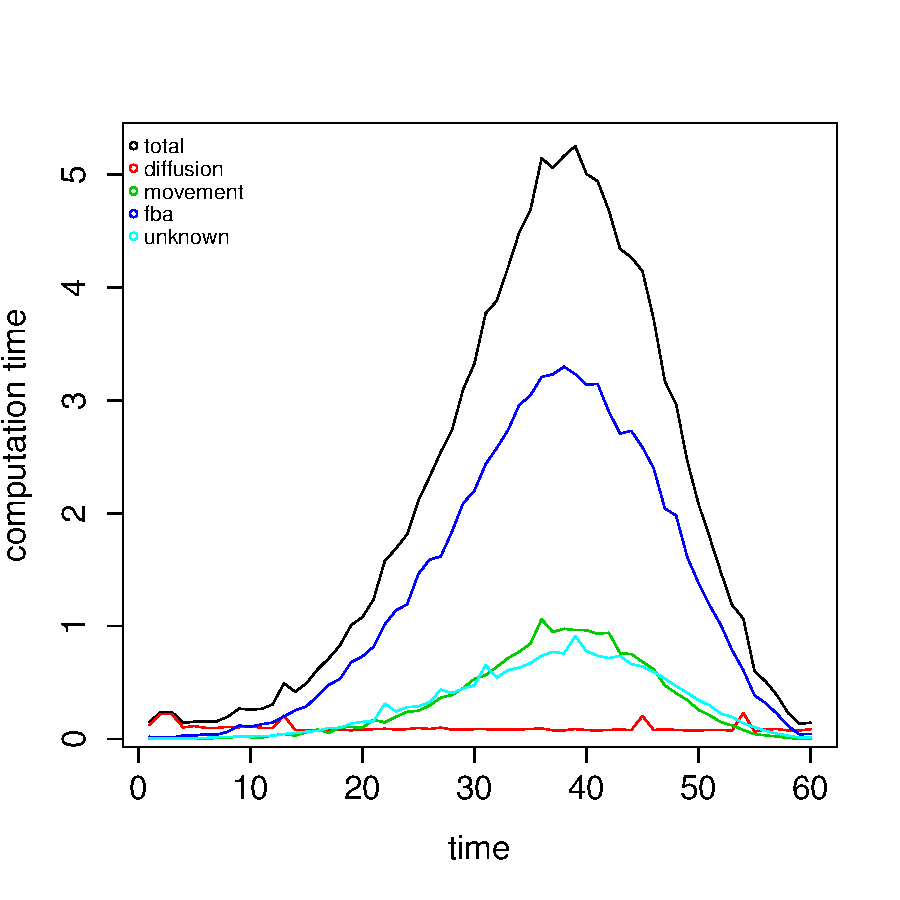
\includegraphics[width=\textwidth]{../results/img/ecoli_20x20_aerob_seed55_time_abs.pdf}
  \end{minipage}
  }
  \subfigure[]{
  \begin{minipage}[t]{0.45\textwidth}
    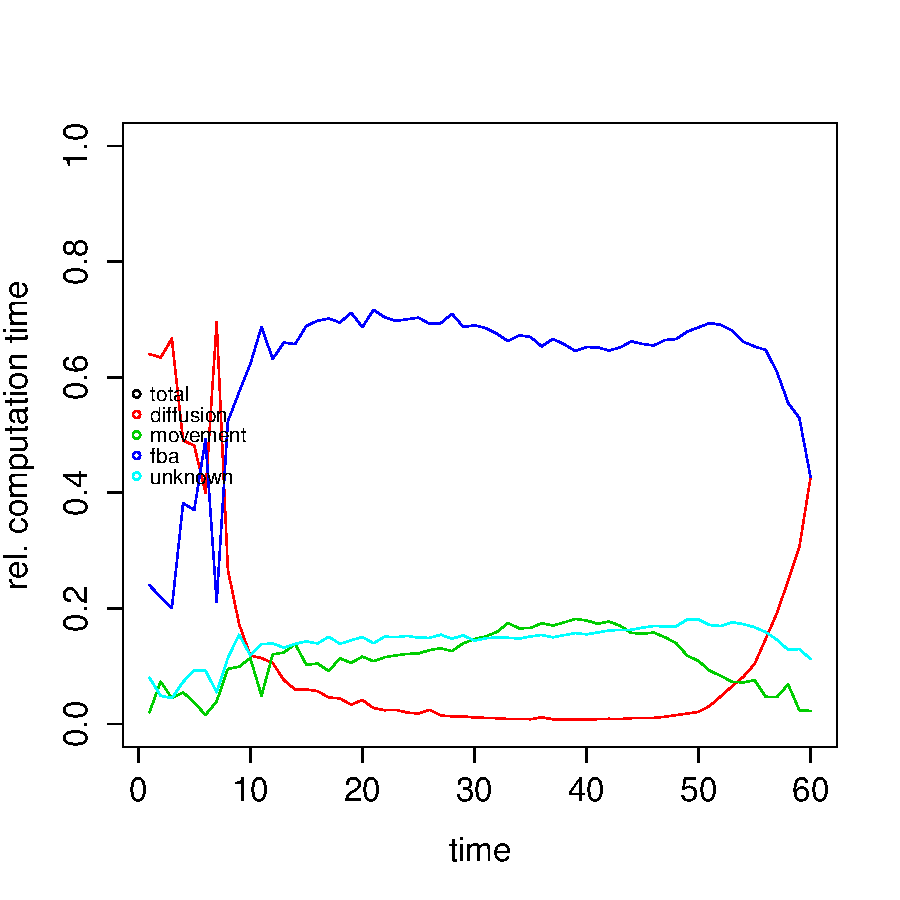
\includegraphics[width=\textwidth]{../results/img/ecoli_20x20_aerob_seed55_time_rel.pdf}
  \end{minipage}
  }
  \caption{Absolute (A) and relative (B) time consumption over the simulation of the \emph{E. coli} core model on a $20 \times 20$ grid.}
  \label{fig:time}
\end{figure}

Considering the time consumption of the whole framework (Figure \hyperref[fig:time]{\ref{fig:time}}), the calculation of the flux balance analysis required the highest amount of time.
Furthermore, the overall fba calculation time was dependent on the number of microbe individuals on the grid, whereat higher numbers of agents resulted in higher overall calculation times. The same was true for the movement function, which consumed after the fba the highest amount of time. The time consumption of diffusion function was considerably lower than the other functions and constant over the whole simulation, since it is independent on the number of microbes on the grid. Other
calculations for diverse matrix operations (primary $x$apply code in \textit{R}) required with respect to the movement a comparable small amount of time, but is significant, too.\\
Grid size was the dominant factor, because bigger space increased the needed time of all other parts: More diffusion, more bacteria, more movement, more fba.
For larger \textit{SBML} models the fba calculations consumed more time.
That's why the amount of metabolic reactions is only relevant for fba calculations.
The time consumption of the other function was independent on the used model and relativly insignificant for \textit{SBML} models taller than $500\times 500$ (reactions $\times$ metabolites).
Therefore, fba was the time limiting factor of the simulations.

\subsection{Population models}

\subsubsection{\textit{Escherichia coli} core}
The \textit{E. coli} core model was subjected to initial concentrations of the substrates glucose and oxygen to generate a population model and monitor the production/consumption of various metabolites (Figure \hyperref[fig:ecoresg]{\ref{fig:ecoresg}}). In the first time steps oxygen and glucose were consumed and CO$_2$ was produced. Additionally, fermentation products such as acetate, formate and ethanol were produced, which increased in concentration during the exponential phase of microbial growth. 
Acetate and formate were produced on high levels (averaged grid cell concentration of $> 60\, mmol$).
That's even more than CO$_2$ ($\approx 50\, mmol$).
The doubling time in the exponential phase was estimated as 7 iteration (h).
The population growth reached the stationary phase after 30 iterations (h), after all substrates were consumed. In the subsequent death phase no metabolites were produced or consumed.
According the dispersion of the microbes on the grid environment, substrates were consumed and metabolites produced (Figure \hyperref[fig:ecoregrids]{\ref{fig:ecoregrids}}).
\begin{figure}[h!]
  \centering
  \subfigure[]{
  %\begin{minipage}[t]{0.45\textwidth}
    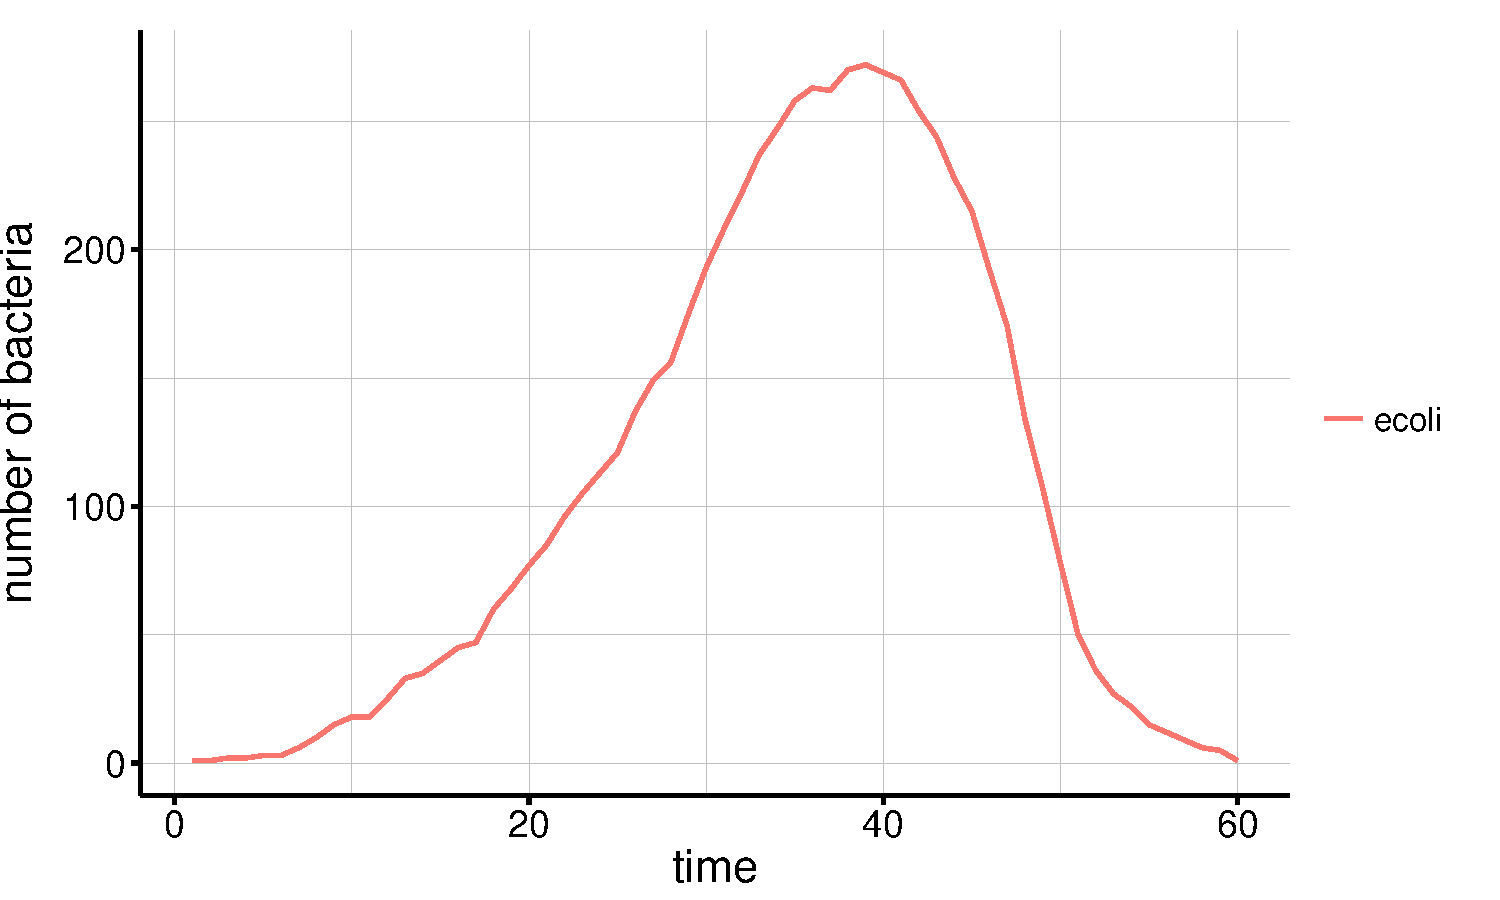
\includegraphics[scale=0.45]{../results/img/ecoli_20x20_aerob_seed55_growth.pdf}
  %\end{minipage}
  }
  \subfigure[]{
  %\begin{minipage}[t]{0.45\textwidth}
    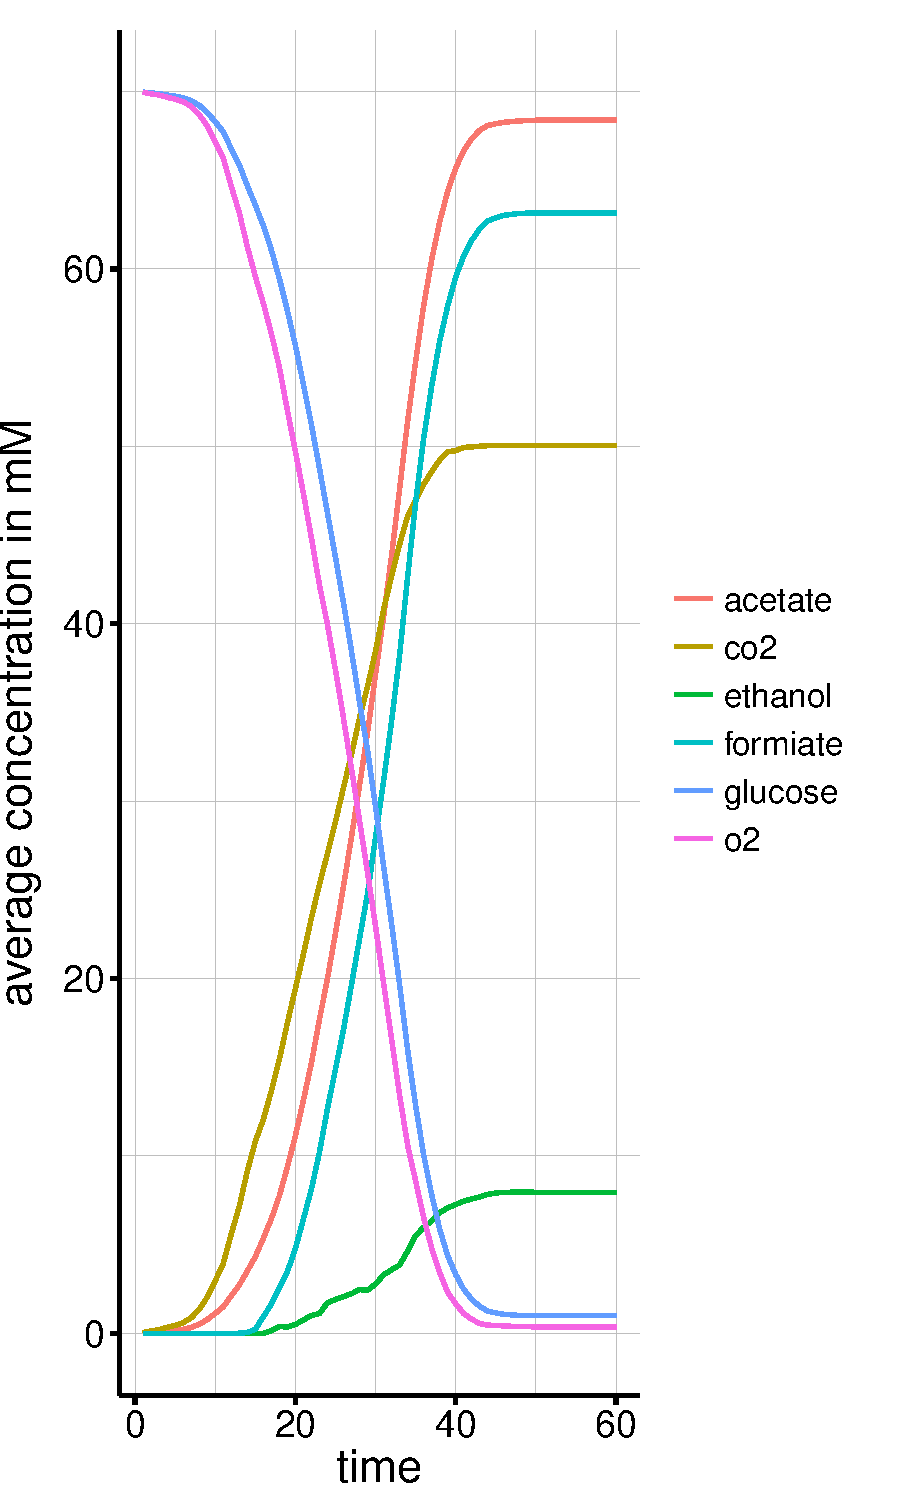
\includegraphics[scale=0.45]{../results/img/ecoli_20x20_aerob_seed55_subs.pdf}
  %\end{minipage}
  }
  \caption{Population dynamics of the \emph{E. coli} core model on a $20\times20$ grid, with bacterial growth (A) and consumption/production of various metabolites (B). An initial concentration of 70\;mmol per grid cell of glucose and oxygen was added to the environment. The seed of the random number generator was set to 55.}
\label{fig:ecoresg}
\end{figure}
\begin{figure}[h!]
  \centering
  \subfigure[]{
    \begin{minipage}[t]{0.3\textwidth}
    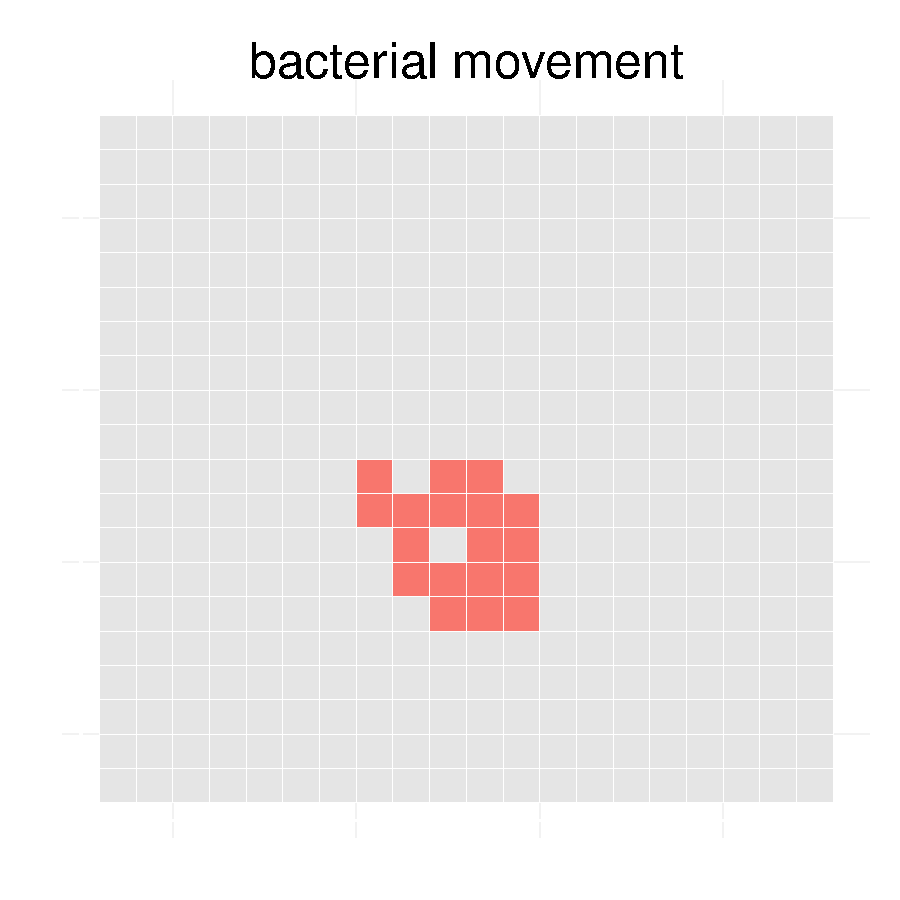
\includegraphics[width=\textwidth]{../results/img/ecoli_20x20_aerob_seed55_bac10.pdf}
  \end{minipage}
  \begin{minipage}[t]{0.3\textwidth}
    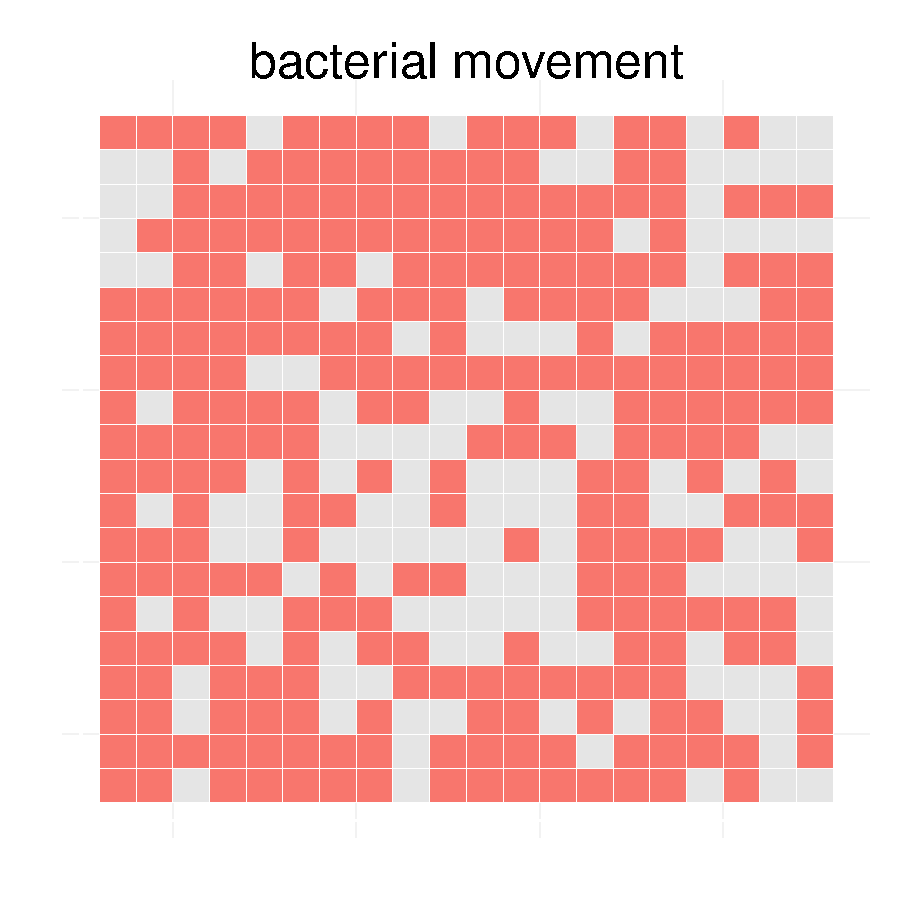
\includegraphics[width=\textwidth]{../results/img/ecoli_20x20_aerob_seed55_bac40.pdf}
  \end{minipage}
  \begin{minipage}[t]{0.3\textwidth}
    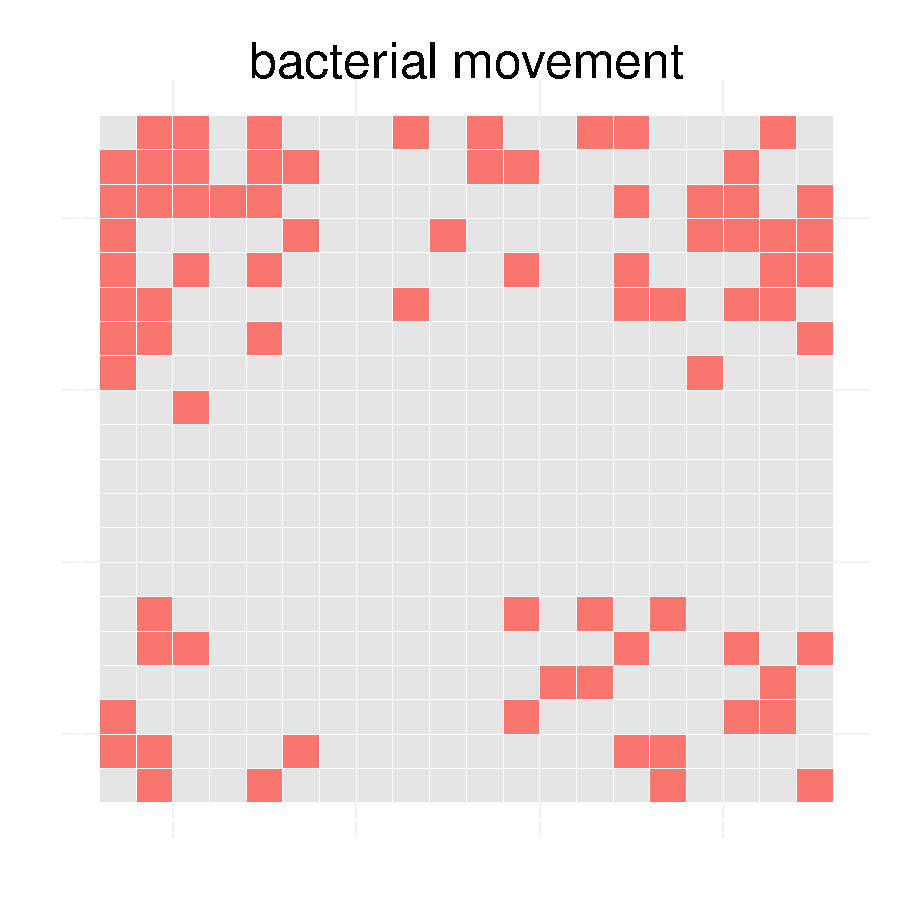
\includegraphics[width=\textwidth]{../results/img/ecoli_20x20_aerob_seed55_bac50.pdf}
  \end{minipage}
  }
  \subfigure[]{
  \begin{minipage}[t]{0.3\textwidth}
    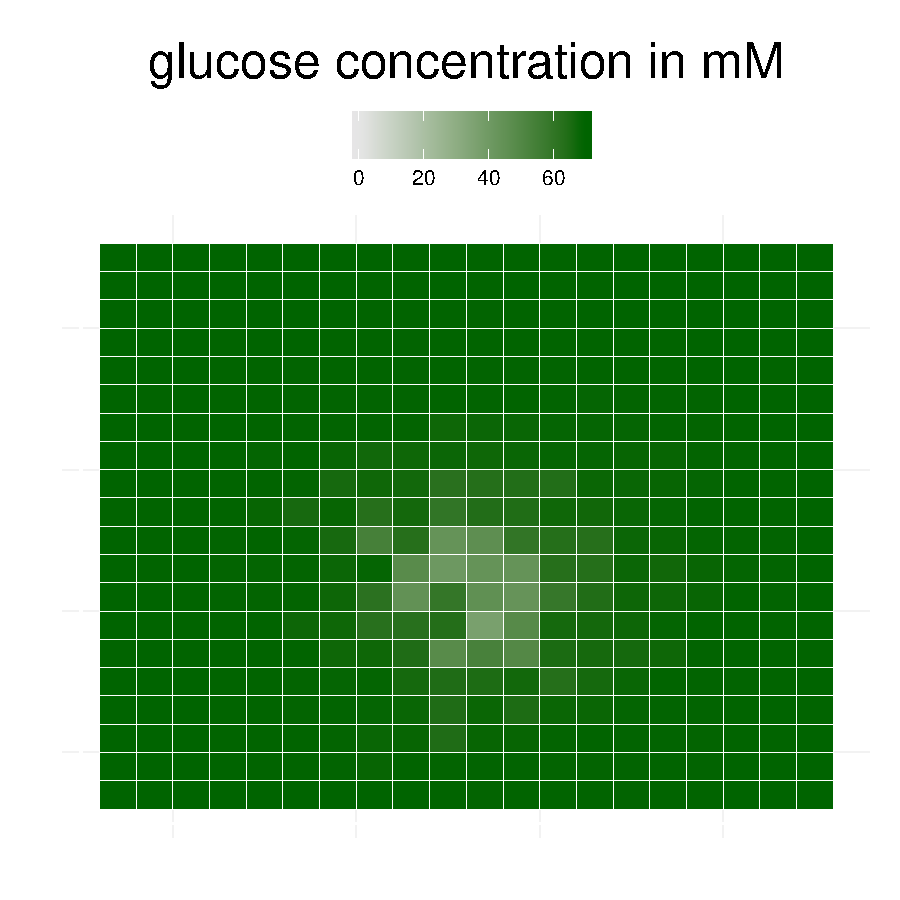
\includegraphics[width=\textwidth]{../results/img/ecoli_20x20_aerob_seed55_glc10.pdf}
  \end{minipage}
  \begin{minipage}[t]{0.3\textwidth}
    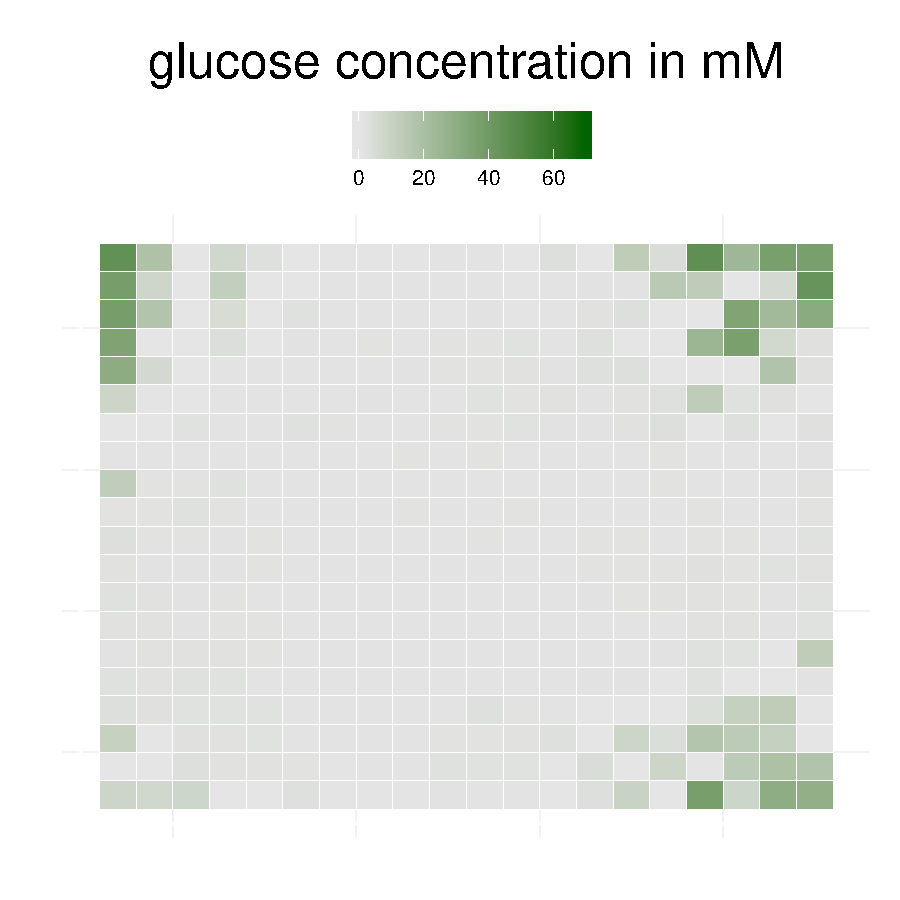
\includegraphics[width=\textwidth]{../results/img/ecoli_20x20_aerob_seed55_glc40.pdf}
  \end{minipage}
  \begin{minipage}[t]{0.3\textwidth}
    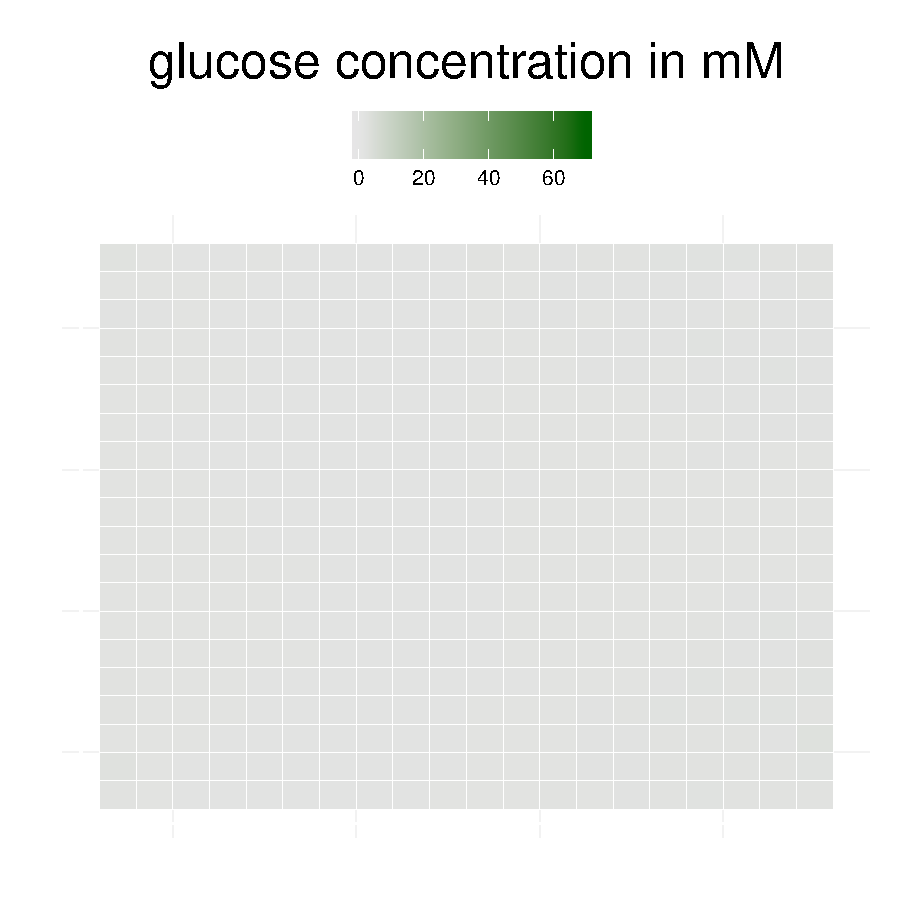
\includegraphics[width=\textwidth]{../results/img/ecoli_20x20_aerob_seed55_glc50.pdf}
  \end{minipage}
  }
  \subfigure[]{
  \begin{minipage}[t]{0.3\textwidth}
    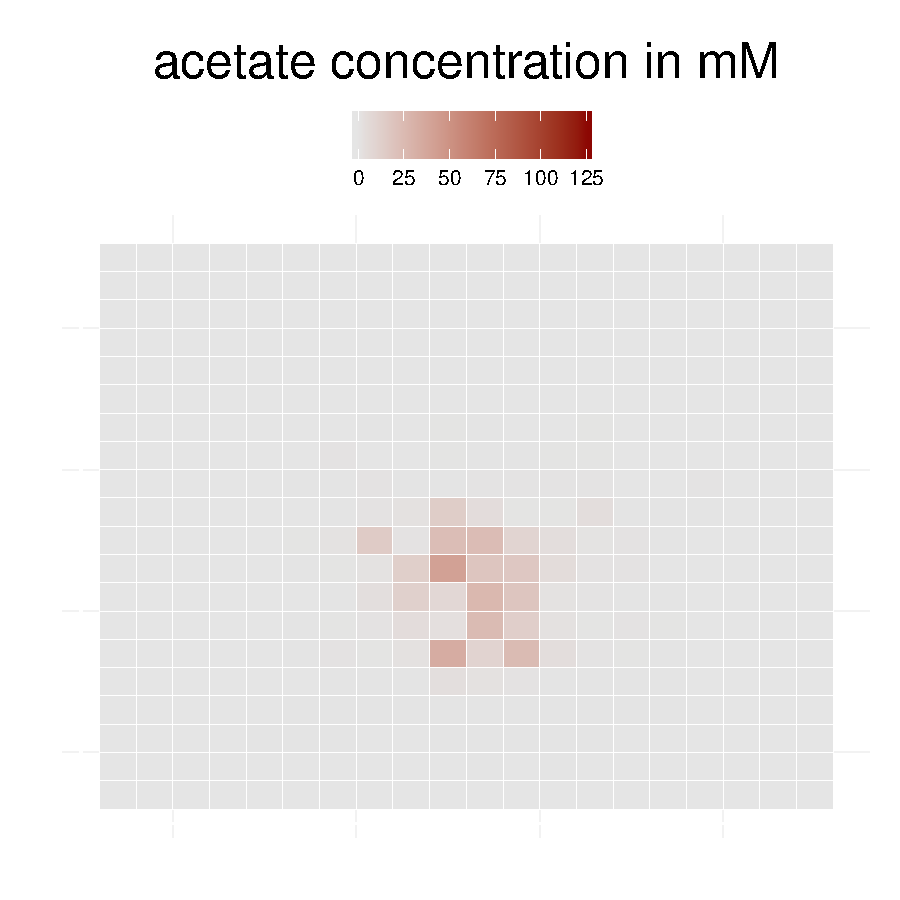
\includegraphics[width=\textwidth]{../results/img/ecoli_20x20_aerob_seed55_ace10.pdf}
  \end{minipage}
  \begin{minipage}[t]{0.3\textwidth}
    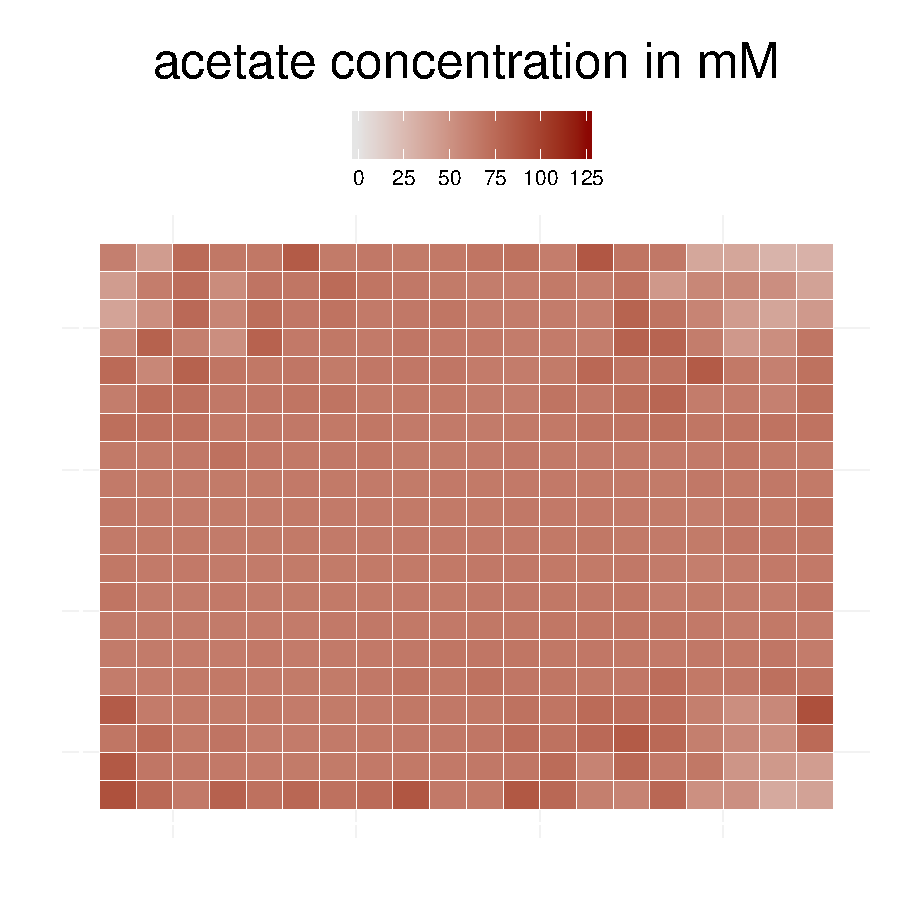
\includegraphics[width=\textwidth]{../results/img/ecoli_20x20_aerob_seed55_ace40.pdf}
  \end{minipage}
  \begin{minipage}[t]{0.3\textwidth}
    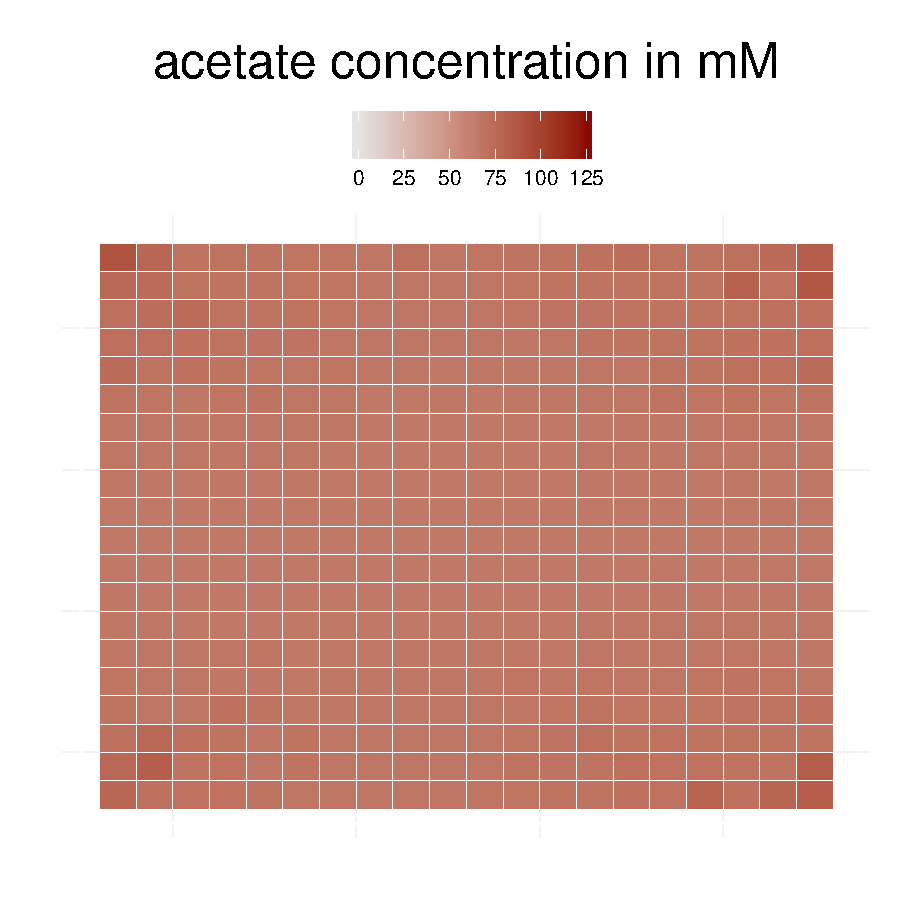
\includegraphics[width=\textwidth]{../results/img/ecoli_20x20_aerob_seed55_ace50.pdf}
  \end{minipage}
  }
  \subfigure[]{
  \begin{minipage}[t]{0.3\textwidth}
    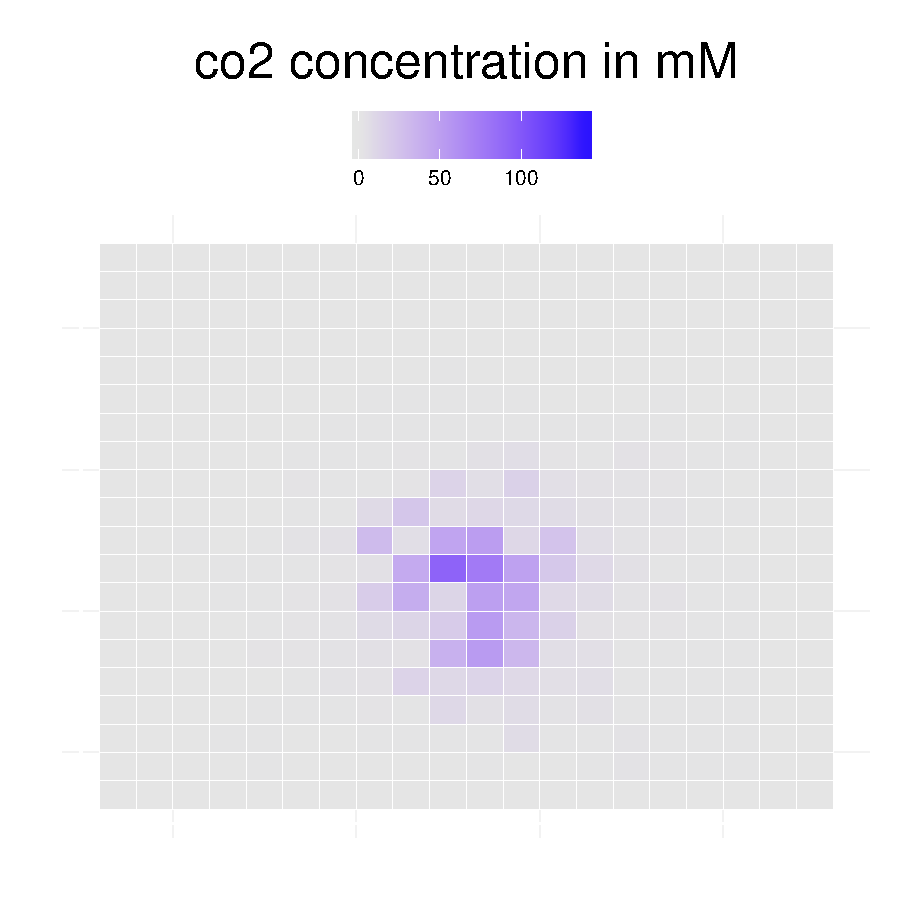
\includegraphics[width=\textwidth]{../results/img/ecoli_20x20_aerob_seed55_co210.pdf}
  \end{minipage}
  \begin{minipage}[t]{0.3\textwidth}
    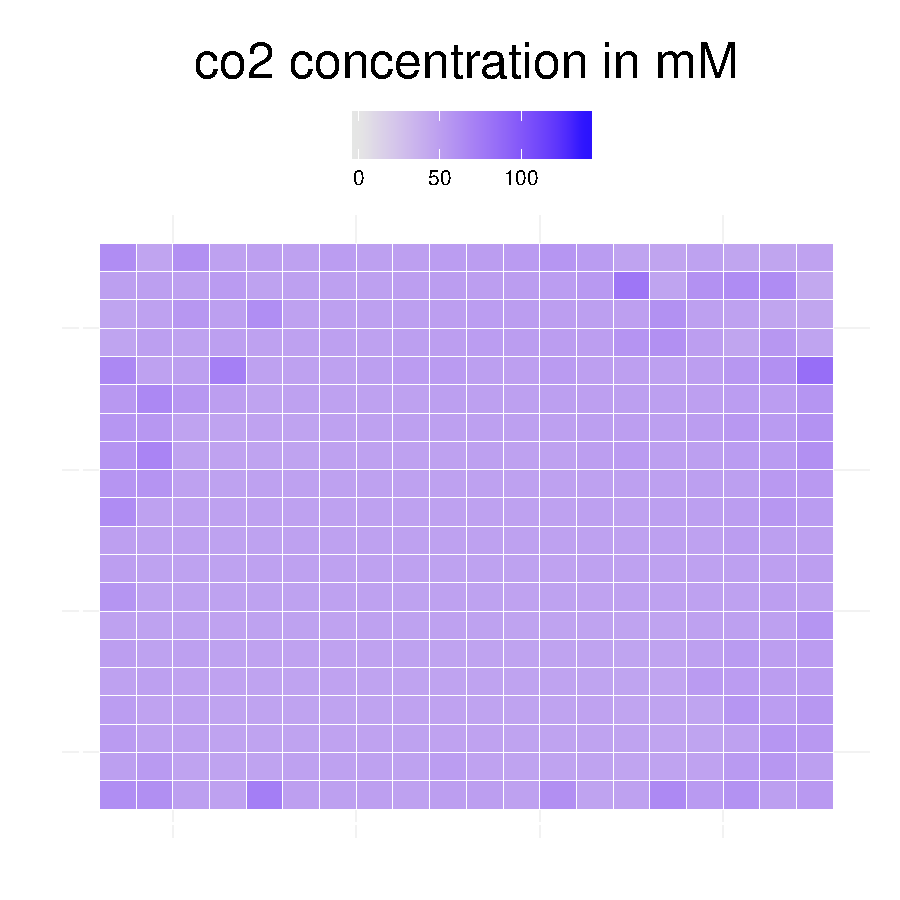
\includegraphics[width=\textwidth]{../results/img/ecoli_20x20_aerob_seed55_co240.pdf}
  \end{minipage}
  \begin{minipage}[t]{0.3\textwidth}
    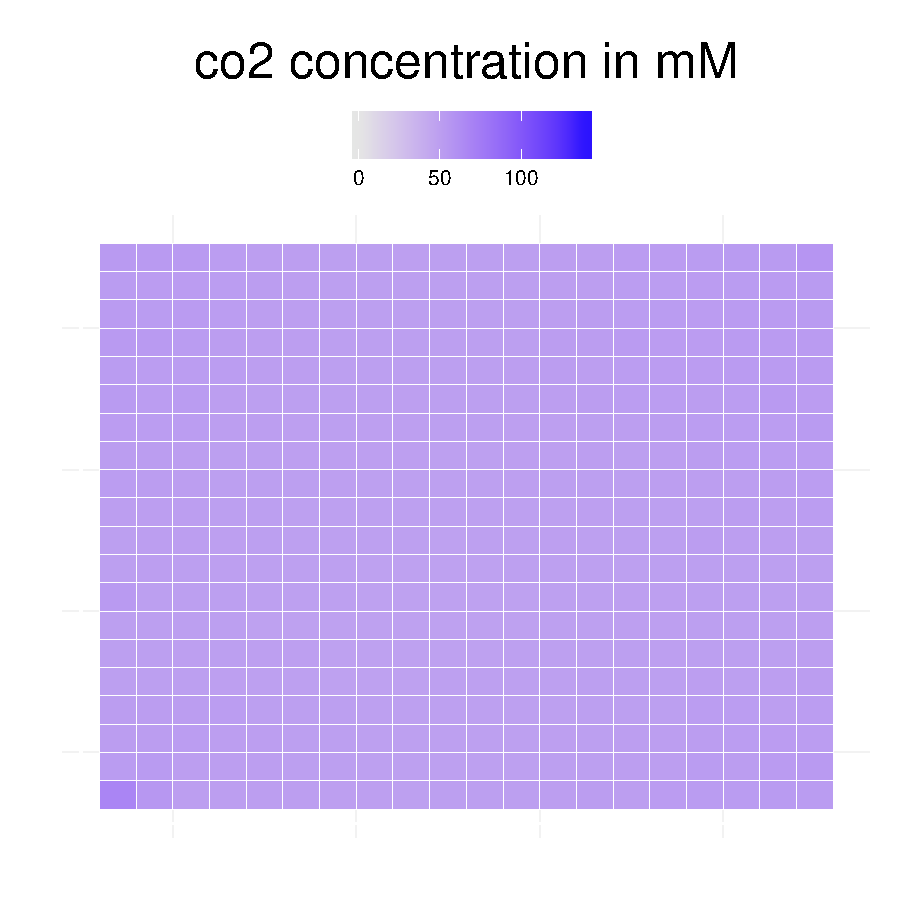
\includegraphics[width=\textwidth]{../results/img/ecoli_20x20_aerob_seed55_co250.pdf}
  \end{minipage}
  }
  %\caption{Population and metabolite dynamics of the \emph{E. coli} core model on a $20\times20$ grid.}
  \caption{Population dynamics of the \emph{E. coli} core model on a $20\times20$ grid, with bacterial movement (A) and concentrations of glucose (B), acetate (C) and CO$_2$ (D) (of time step 10, 40 and 50). The seed of the random number generator was set to 55.}
  \label{fig:ecoregrids}
\end{figure}

\subsubsection{\textit{Escherichia coli big (,,Bcoli'')}}
The \textit{E. coli} model was subjected to initial concentrations of the substrates glucose and oxygen to generate a population model and monitor the production/consumption of various metabolites (Figure \hyperref[fig:ecolisg]{\ref{fig:ecolisg}}). In the first time steps oxygen and glucose were consumed and CO$_2$ was produced. Additionally, few time steps later fermentation products such as acetate and ethanol were produced, which increased in concentration during the exponential phase of microbial growth. 
CO$_2$ reached average grid cell concentration of $\approx 120\, mmol$, acetate $\approx 50\, mmol$ and ethanol had a final concentration of $\approx 10\,mmol$.
In the simulation, no production of formate was found. The doubling time in the exponential phase was estimated as 6 iteration (h).

The population growth reached the stationary phase in approximately 30 iterations (h), after all substrates were consumed. In the subsequent death phase no metabolites were produced or consumed. The population died out after 60 iterations.

According the dispersion of the microbes on the grid environment, substrates were consumed and metabolites produced (Figure \hyperref[fig:ecoligrids]{\ref{fig:ecoligrids}}). Here, CO$_2$ was produced on every position the bacterial agents visited and  acetate was preferably produced in the centre of the grid.
\begin{figure}[h!]
  \centering
    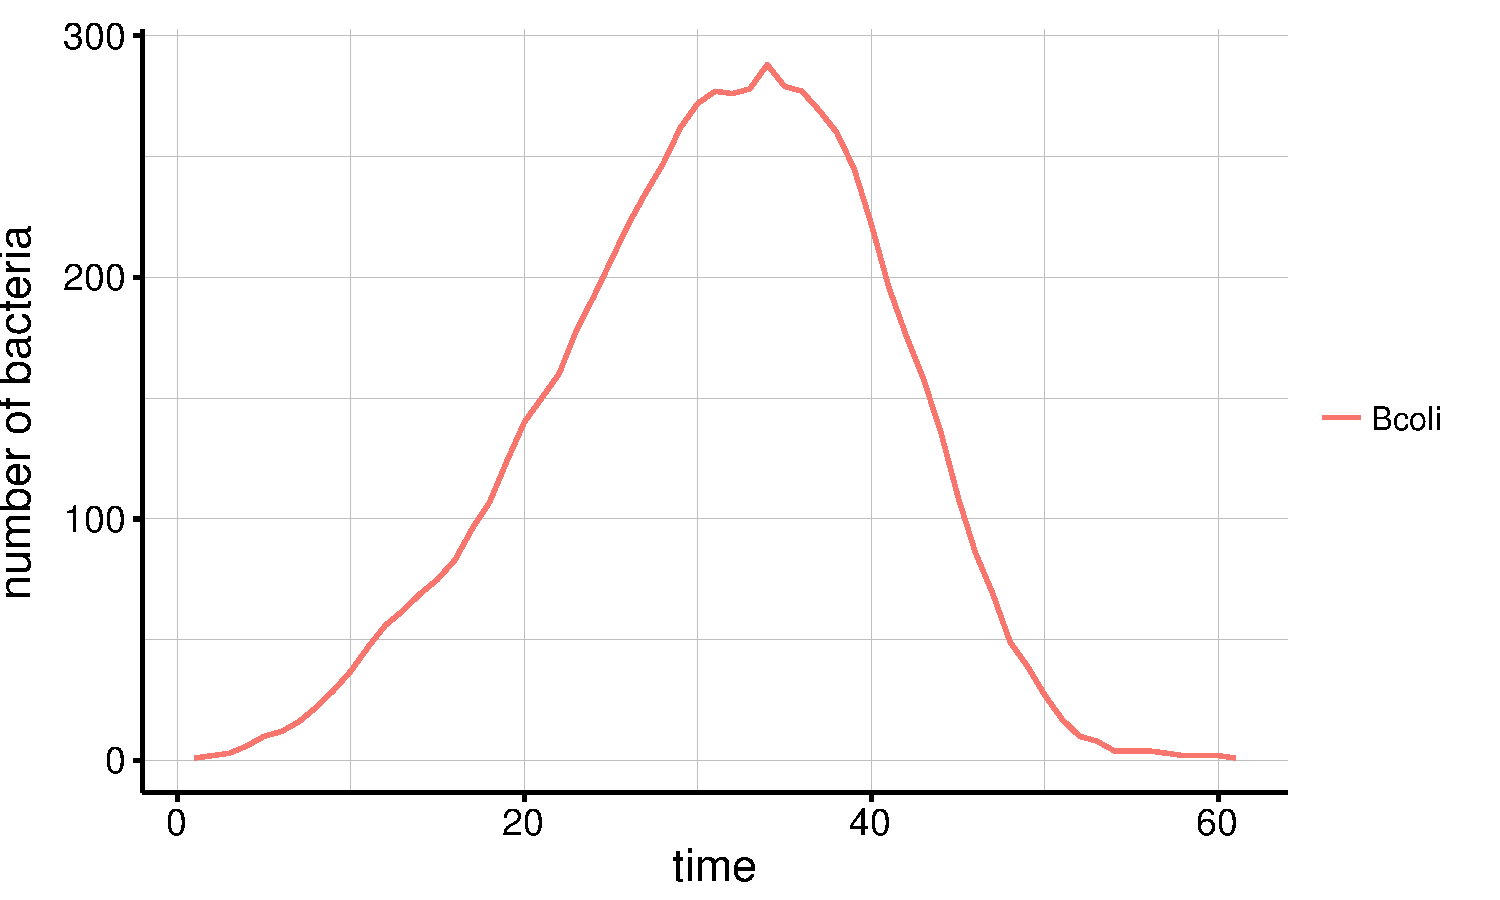
\includegraphics[scale=0.45]{../results/img/Bcoli_20x20_seed176_growth.pdf}
    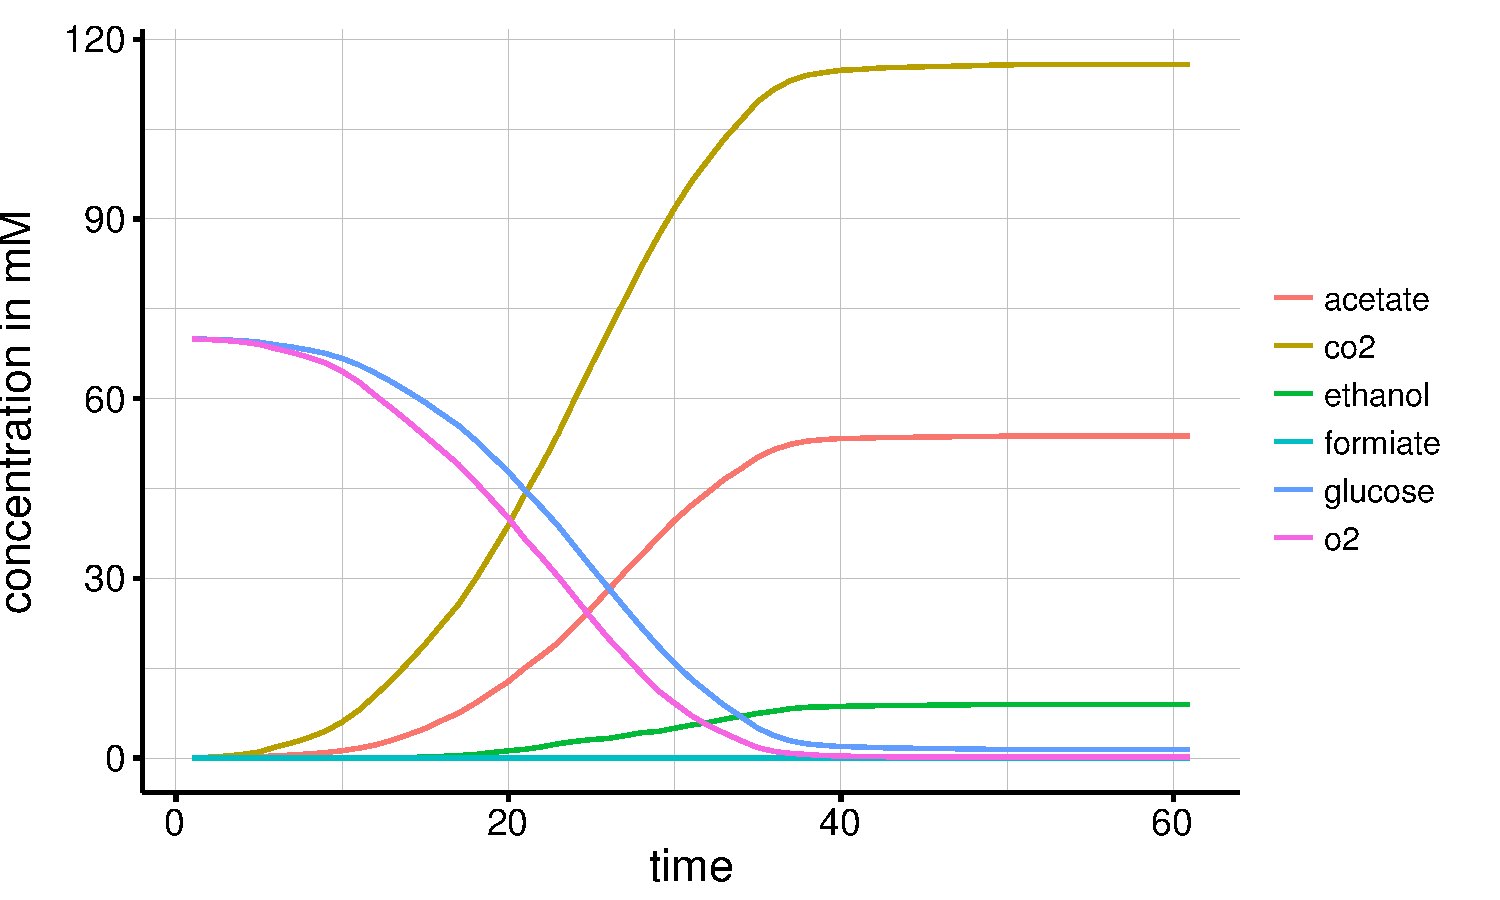
\includegraphics[scale=0.45]{../results/img/Bcoli_20x20_seed176_subs.pdf}
  \caption{Population dynamics of the big \emph{E. coli} model on a $20\times20$ grid, with bacterial growth (A) and consumption/production of various metabolites (B). An initial concentration of 70\;mmol per grid cell of glucose and oxygen was added to the environment. The seed of the random number generator was set to 176.}
  \label{fig:ecolisg}
\end{figure}
\begin{figure}[h!]
  \centering
  \subfigure[]{
    \begin{minipage}[t]{0.3\textwidth}
    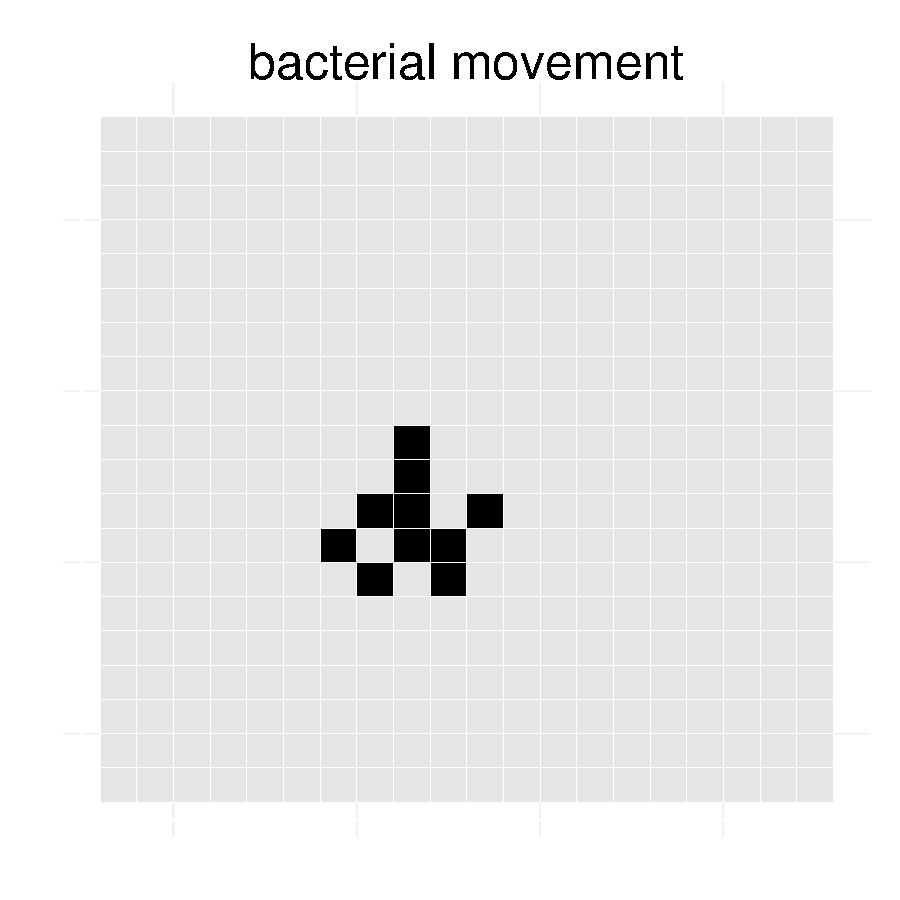
\includegraphics[width=\textwidth]{../results/img/Bcoli_20x20_seed176_bac5.pdf}
  \end{minipage}
  \begin{minipage}[t]{0.3\textwidth}
    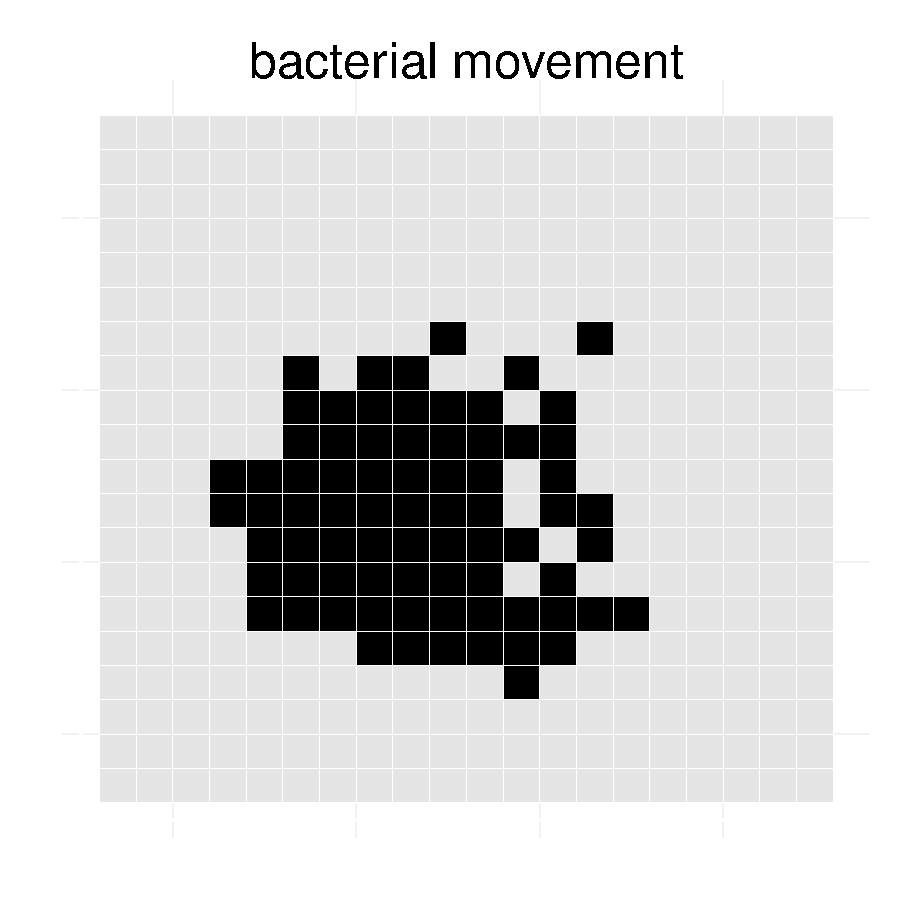
\includegraphics[width=\textwidth]{../results/img/Bcoli_20x20_seed176_bac15.pdf}
  \end{minipage}
  \begin{minipage}[t]{0.3\textwidth}
    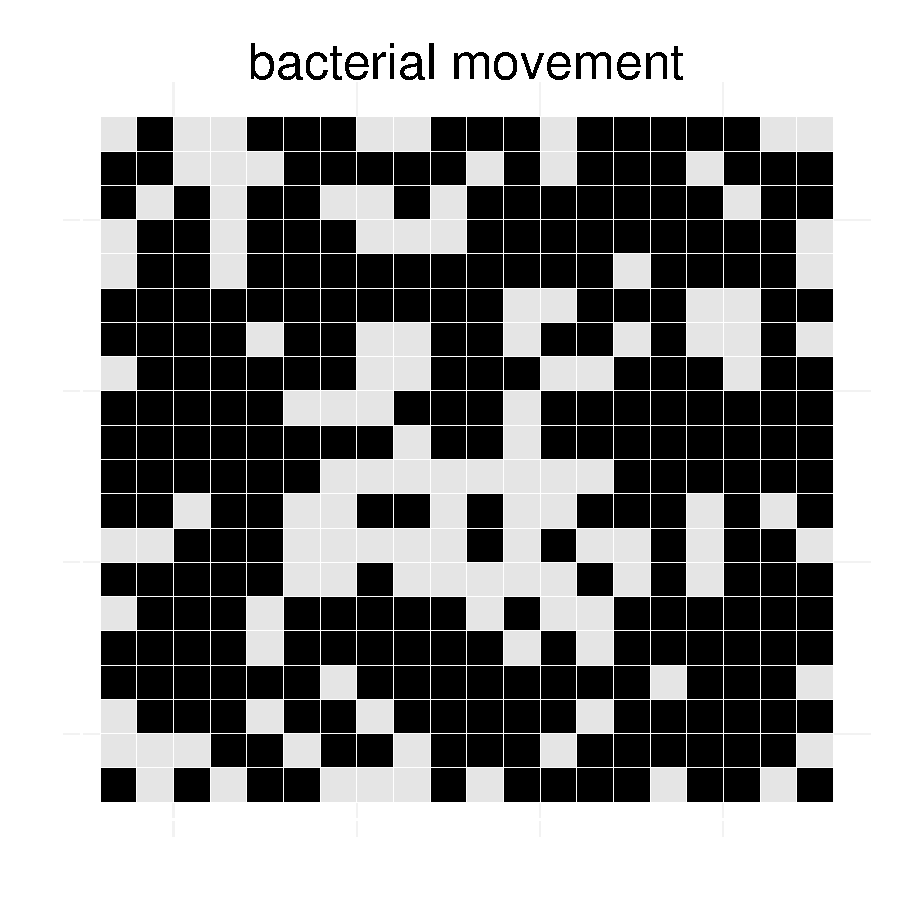
\includegraphics[width=\textwidth]{../results/img/Bcoli_20x20_seed176_bac35.pdf}
  \end{minipage}
  }
  \subfigure[]{
  \begin{minipage}[t]{0.3\textwidth}
    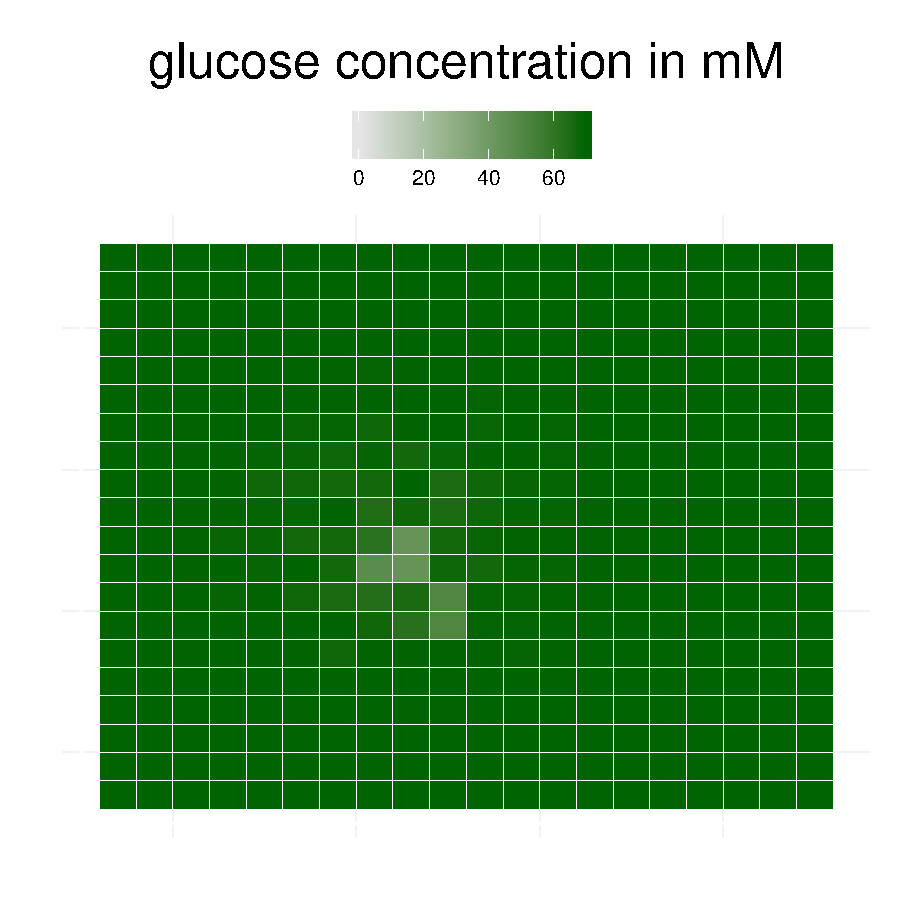
\includegraphics[width=\textwidth]{../results/img/Bcoli_20x20_seed176_glucose5a.pdf}
  \end{minipage}
  \begin{minipage}[t]{0.3\textwidth}
    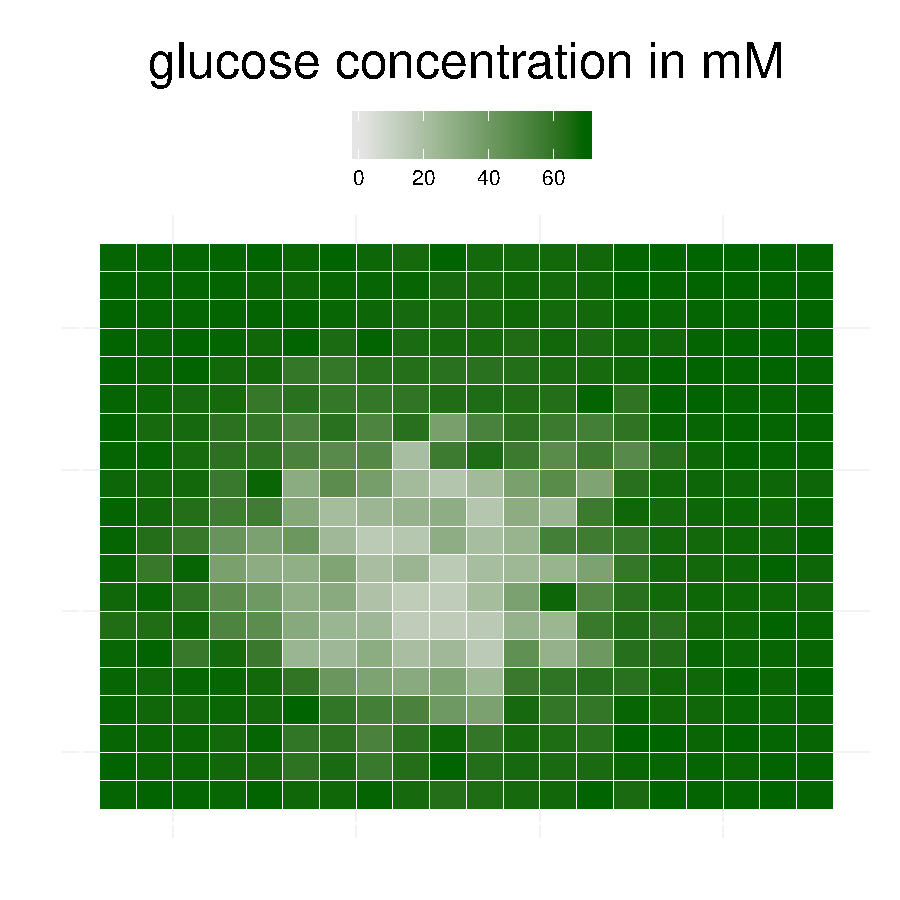
\includegraphics[width=\textwidth]{../results/img/Bcoli_20x20_seed176_glucose15.pdf}
  \end{minipage}
  \begin{minipage}[t]{0.3\textwidth}
    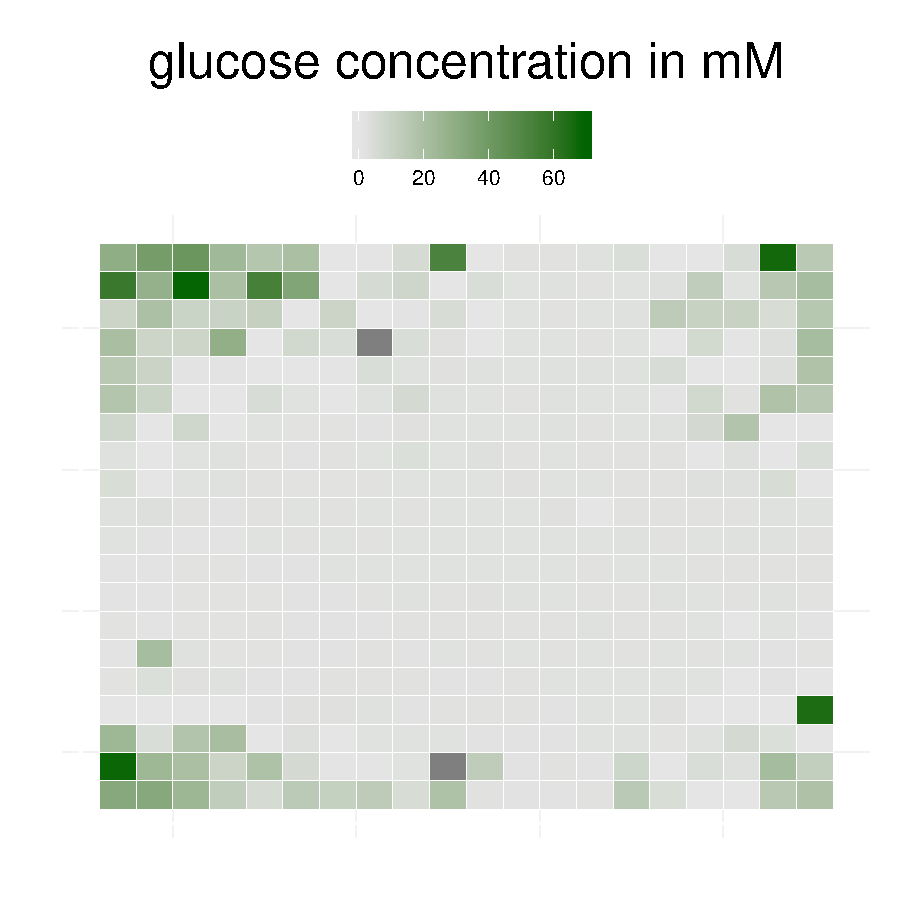
\includegraphics[width=\textwidth]{../results/img/Bcoli_20x20_seed176_glucose35a.pdf}
  \end{minipage}
  }
  \subfigure[]{
  \begin{minipage}[t]{0.3\textwidth}
    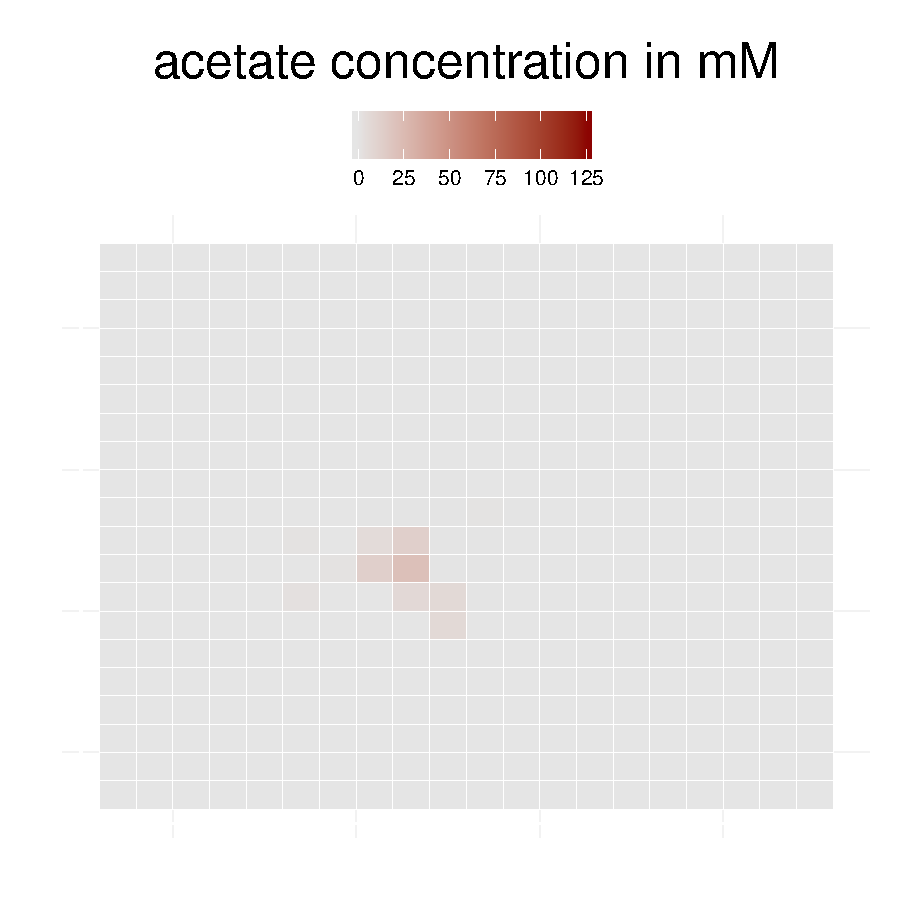
\includegraphics[width=\textwidth]{../results/img/Bcoli_20x20_seed176_ace5a.pdf}
  \end{minipage}
  \begin{minipage}[t]{0.3\textwidth}
    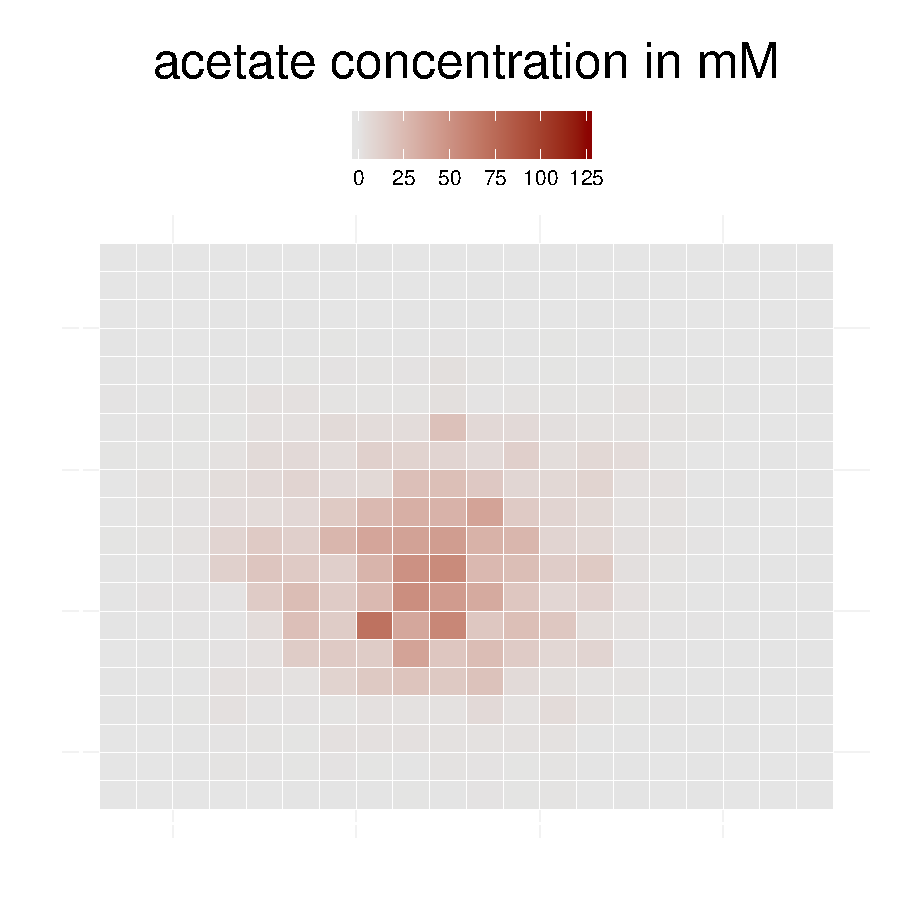
\includegraphics[width=\textwidth]{../results/img/Bcoli_20x20_seed176_ace15.pdf}
  \end{minipage}
  \begin{minipage}[t]{0.3\textwidth}
    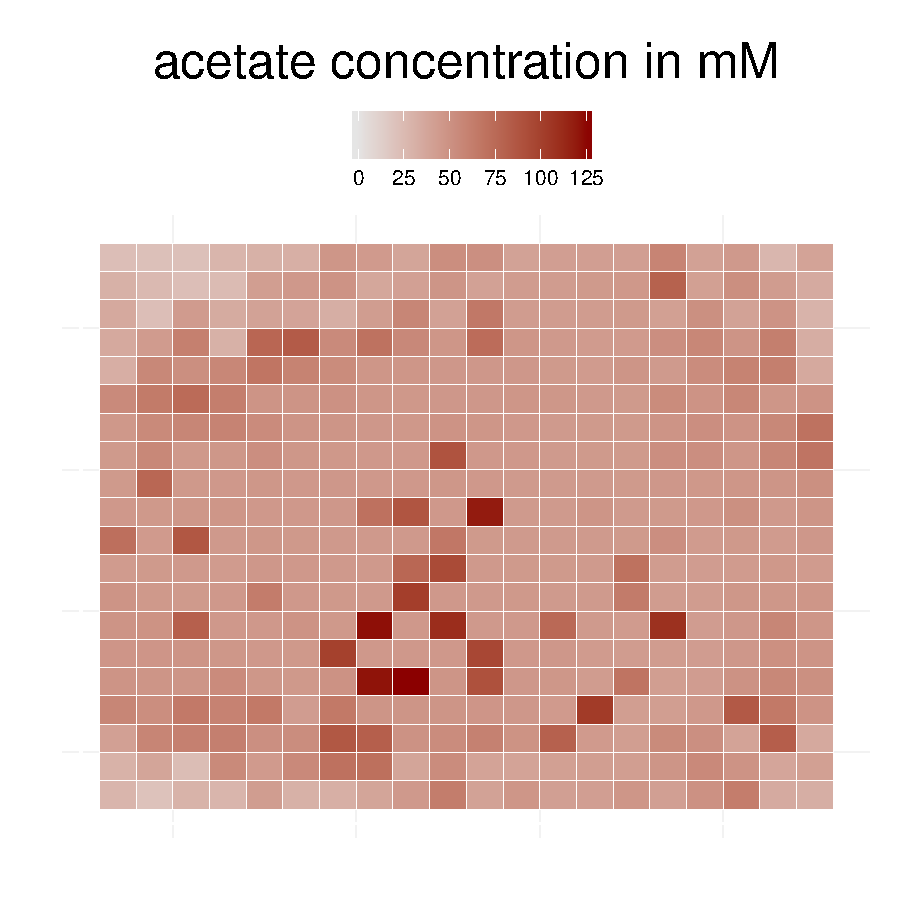
\includegraphics[width=\textwidth]{../results/img/Bcoli_20x20_seed176_ace35a.pdf}
  \end{minipage}
  }
  \subfigure[]{
  \begin{minipage}[t]{0.3\textwidth}
    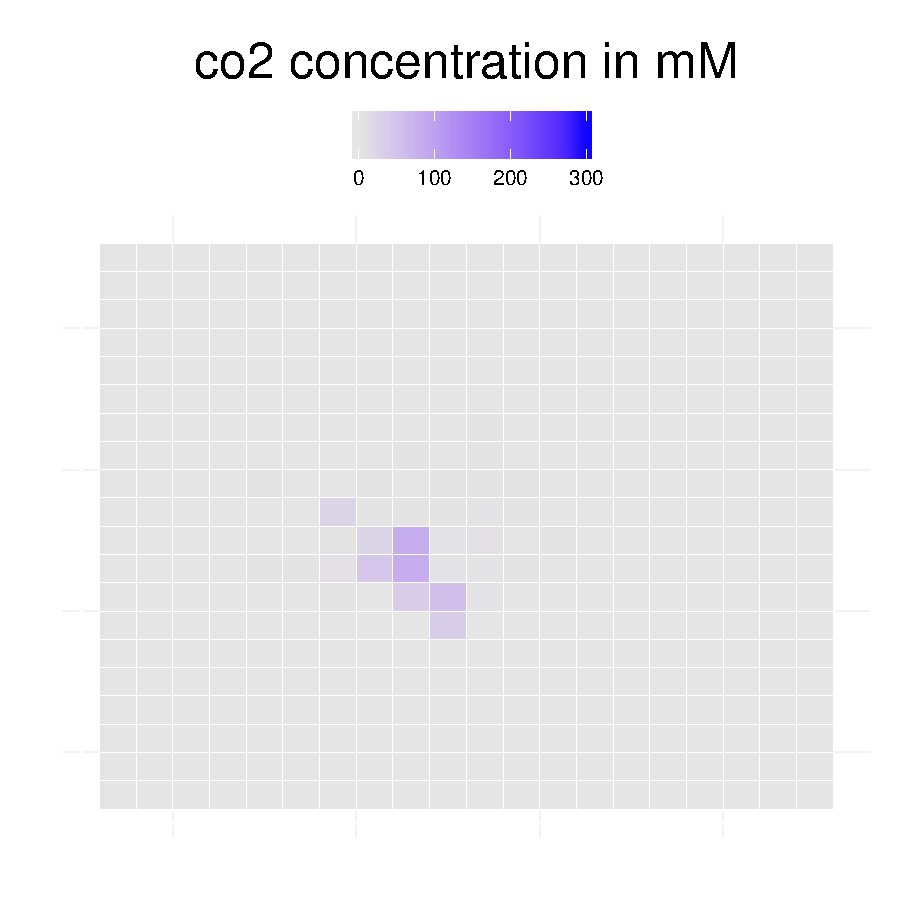
\includegraphics[width=\textwidth]{../results/img/Bcoli_20x20_seed176_co25a.pdf}
  \end{minipage}
  \begin{minipage}[t]{0.3\textwidth}
    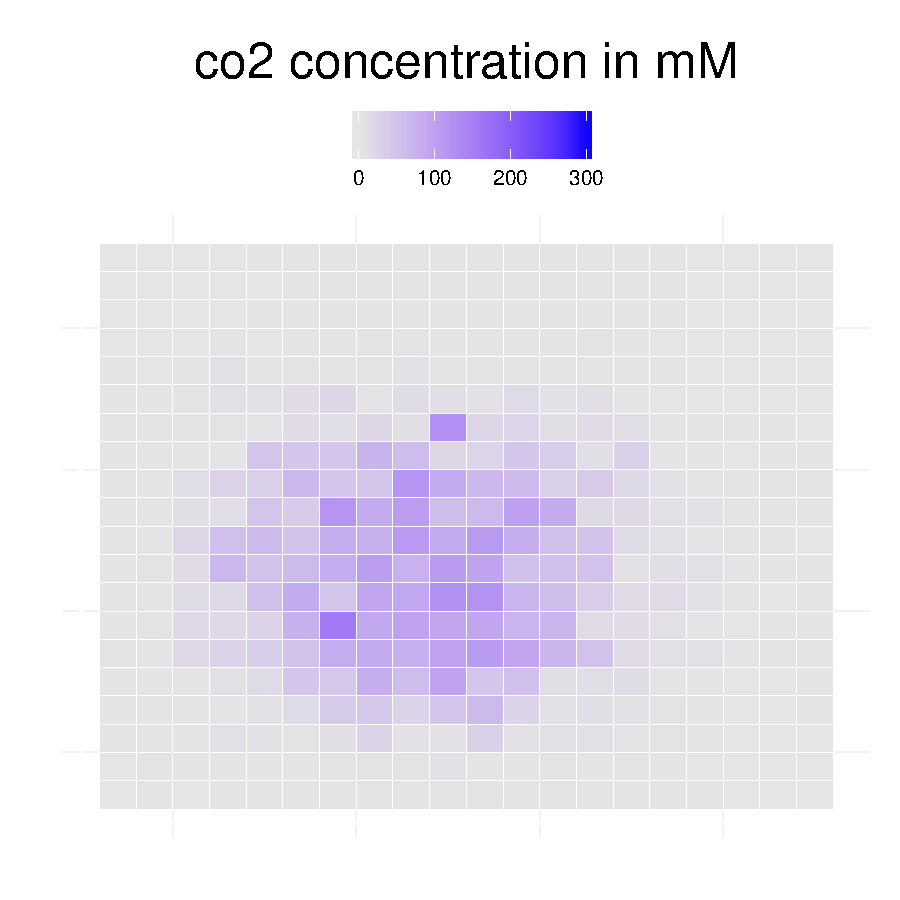
\includegraphics[width=\textwidth]{../results/img/Bcoli_20x20_seed176_co215.pdf}
  \end{minipage}
  \begin{minipage}[t]{0.3\textwidth}
    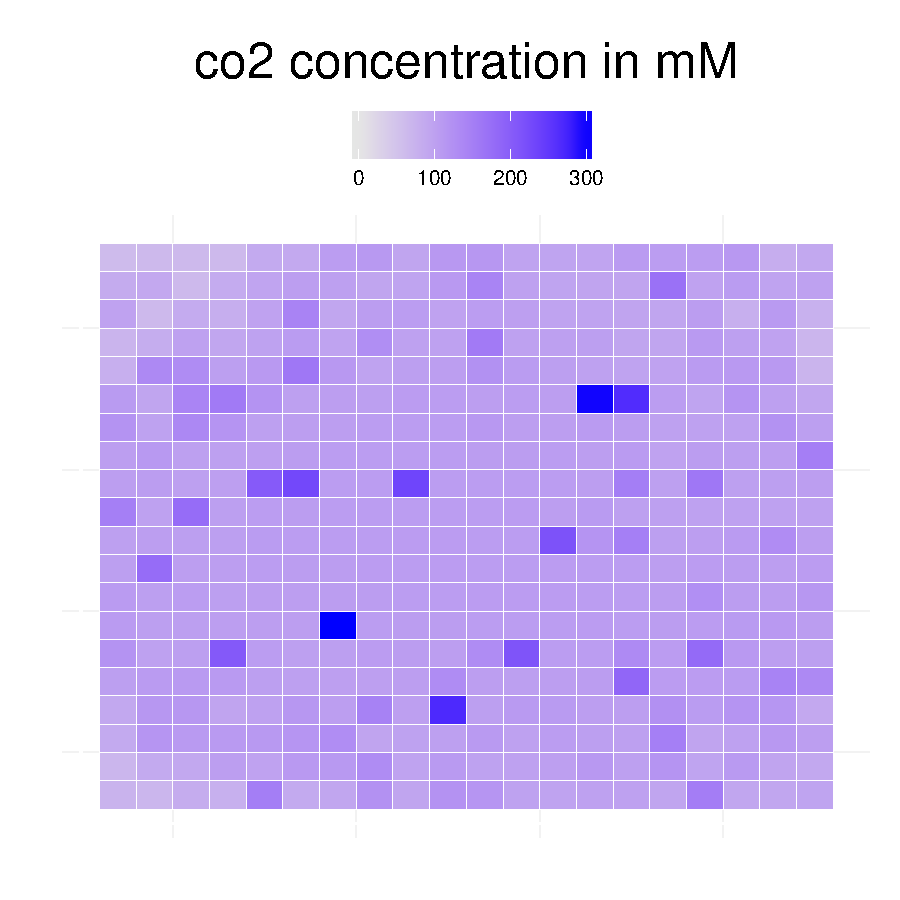
\includegraphics[width=\textwidth]{../results/img/Bcoli_20x20_seed176_co235a.pdf}
  \end{minipage}
  }
  \caption{Population dynamics of the big \emph{E. coli} model on a $20\times20$ grid, with bacterial movement (A) and concentrations of glucose (B), acetate (C) and CO$_2$ (D) (of time step 5, 15 and 35). The seed of the random number generator was set to 176.}
  \label{fig:ecoligrids}
\end{figure}

\subsubsection{\textit{Methanosarcina barkeri}}
The \textit{M. barkeri} model was subjected to initial concentrations of methanol as a substrate, to generate a population model and monitor the production/consumption of various metabolites (Figure \hyperref[fig:barkerisg]{\ref{fig:barkerisg}}). In the first time steps methanol was consumed and CO$_2$, methane and water was produced. Compared to water and methane, the production of CO$_2$ was considerably lower.
The doubling time in the exponential phase was estimated as 17 iteration (h).
The population growth reached the stationary phase in approximately 100 iterations (h), after methanol was consumed. In the subsequent death phase no metabolites were produced or consumed. The population died out after 150 iterations.
According the dispersion of the microbes on the grid environment, substrates were consumed and metabolites produced (Figure \hyperref[fig:barkerigrids]{\ref{fig:barkerigrids}}).
\begin{figure}[h!]
  \centering
    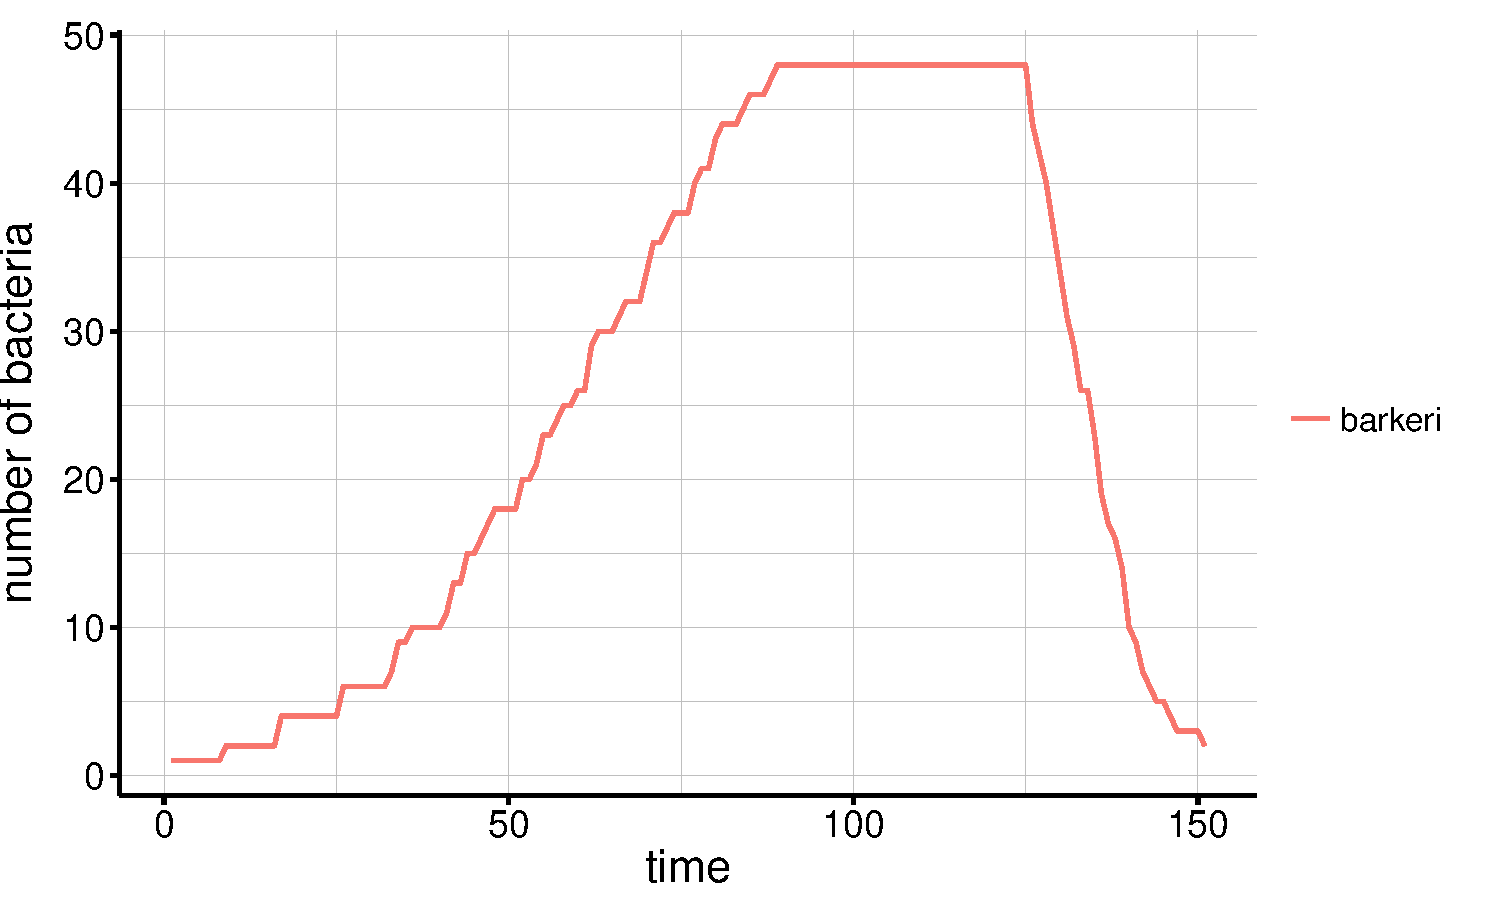
\includegraphics[scale=0.45]{../results/img/barkeri_20x20_seed9659_growth.pdf}
    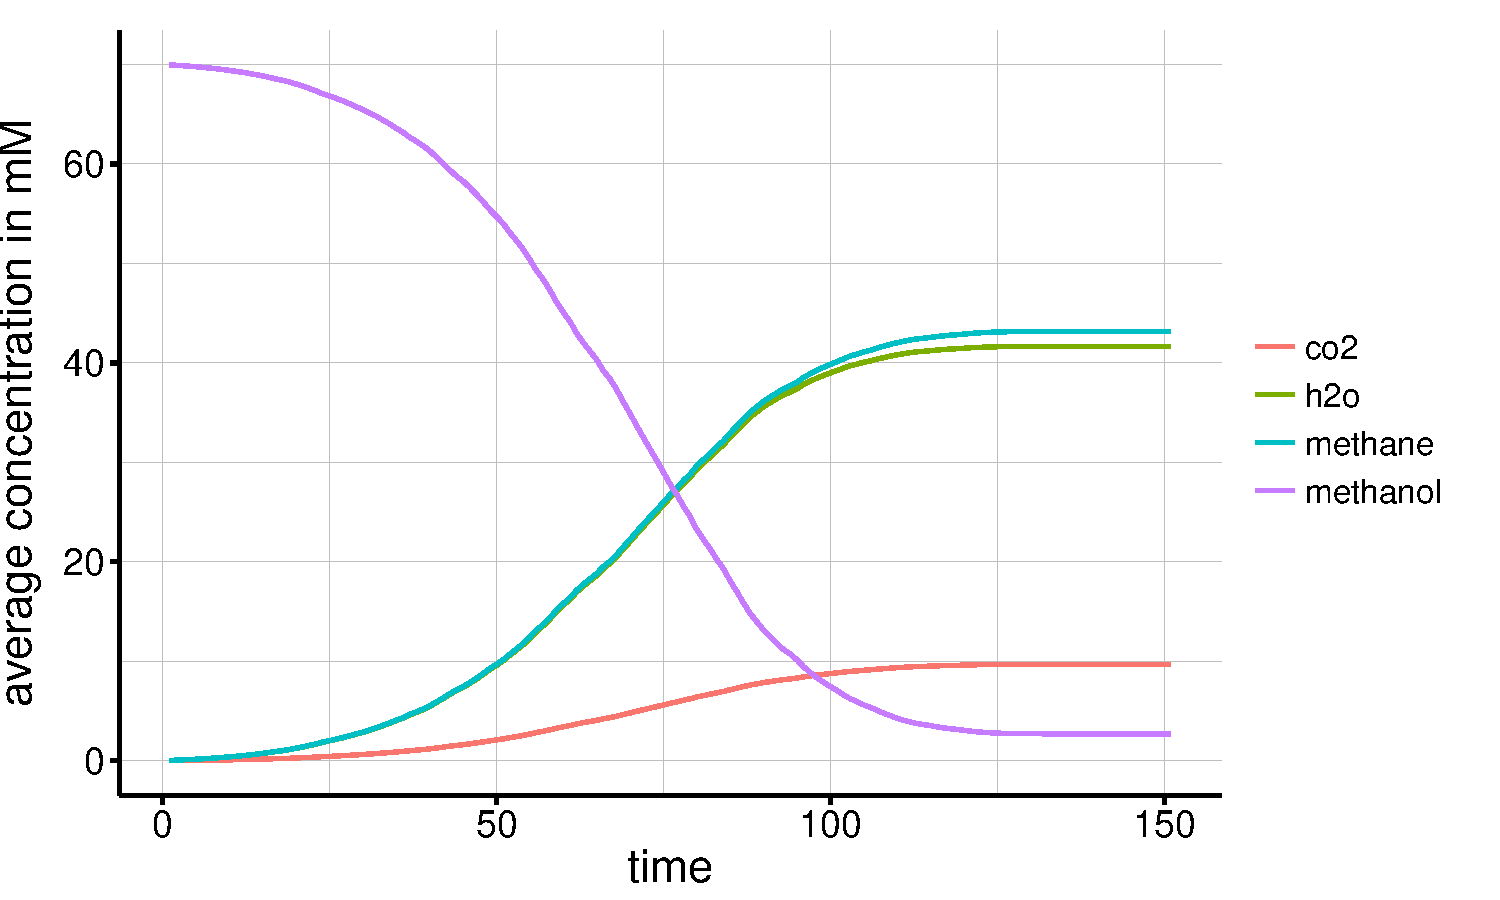
\includegraphics[scale=0.45]{../results/img/barkeri_20x20_seed9659_subs.pdf}
  \caption{Population dynamics of the \emph{M. barkeri} model on a $20\times20$ grid, with bacterial growth (A) and consumption/production of various metabolites (B). An initial concentration of 70\;mmol per grid cell of methanol was added to the environment. The seed of the random number generator was set to 9659.}
  \label{fig:barkerisg}
\end{figure}
\begin{figure}[h!]

  \centering
  \subfigure[]{
    \begin{minipage}[t]{0.3\textwidth}
    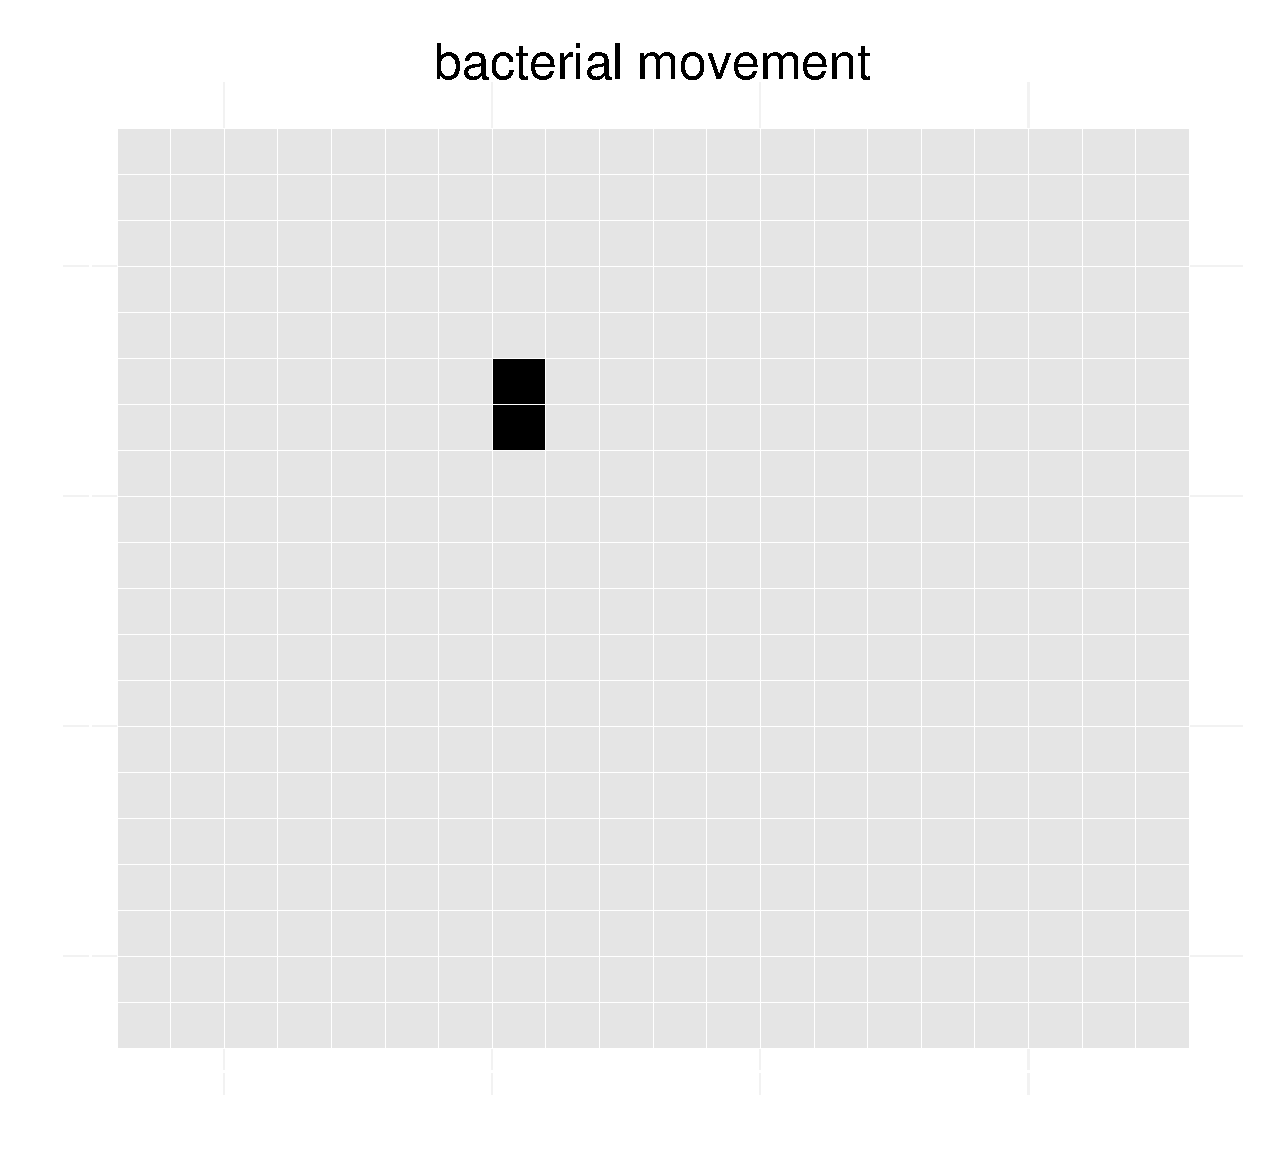
\includegraphics[width=\textwidth]{../results/img/barkeri_20x20_seed9659_bac10.pdf}
  \end{minipage}
  \begin{minipage}[t]{0.3\textwidth}
    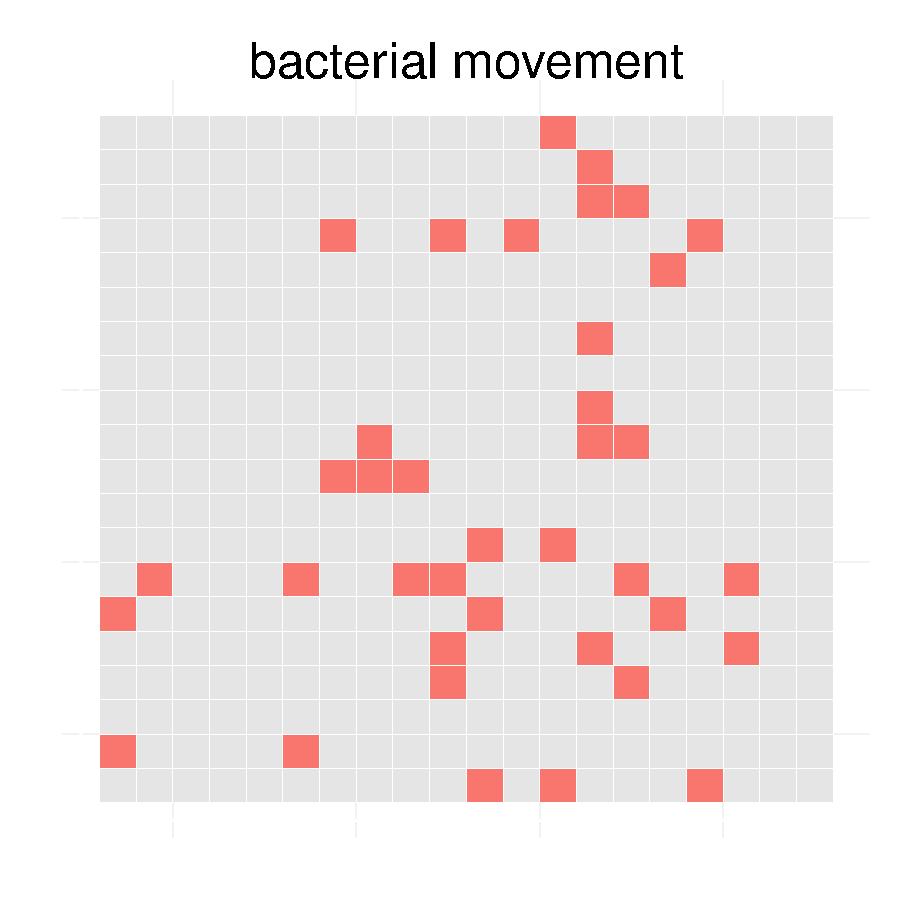
\includegraphics[width=\textwidth]{../results/img/barkeri_20x20_seed9659_bac75.pdf}
  \end{minipage}
  \begin{minipage}[t]{0.3\textwidth}
      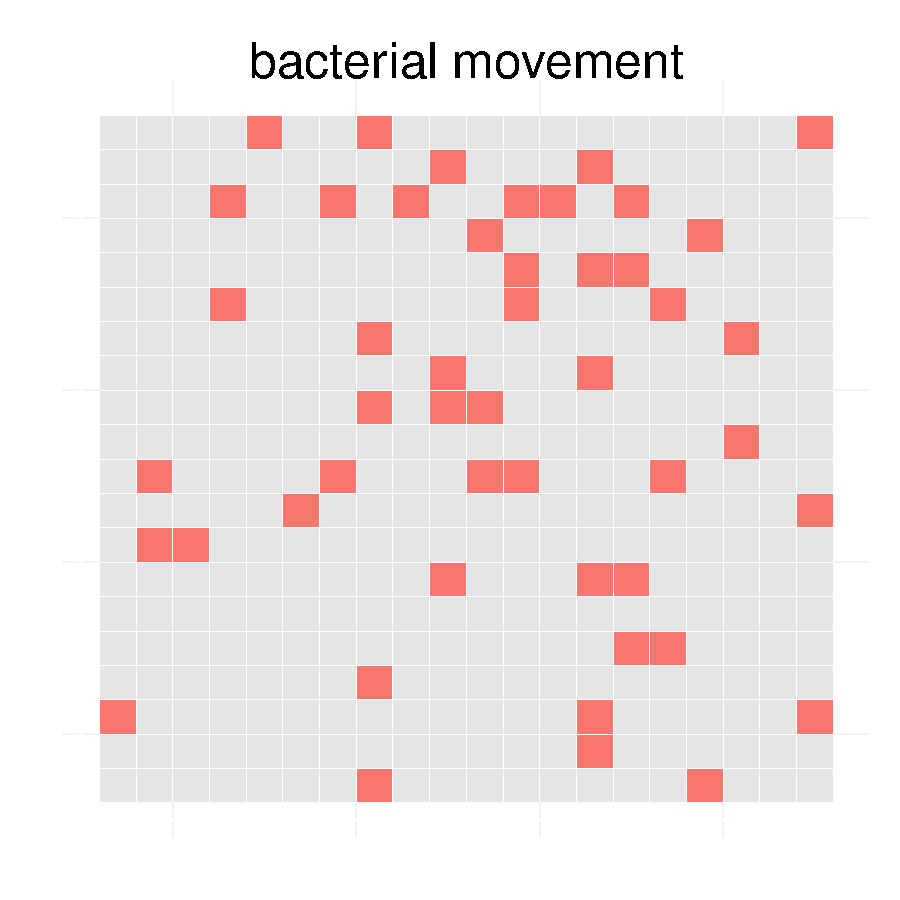
\includegraphics[width=\textwidth]{../results/img/barkeri_20x20_seed9659_bac100.pdf}
  \end{minipage}
  }
  \subfigure[]{
  \begin{minipage}[t]{0.3\textwidth}
    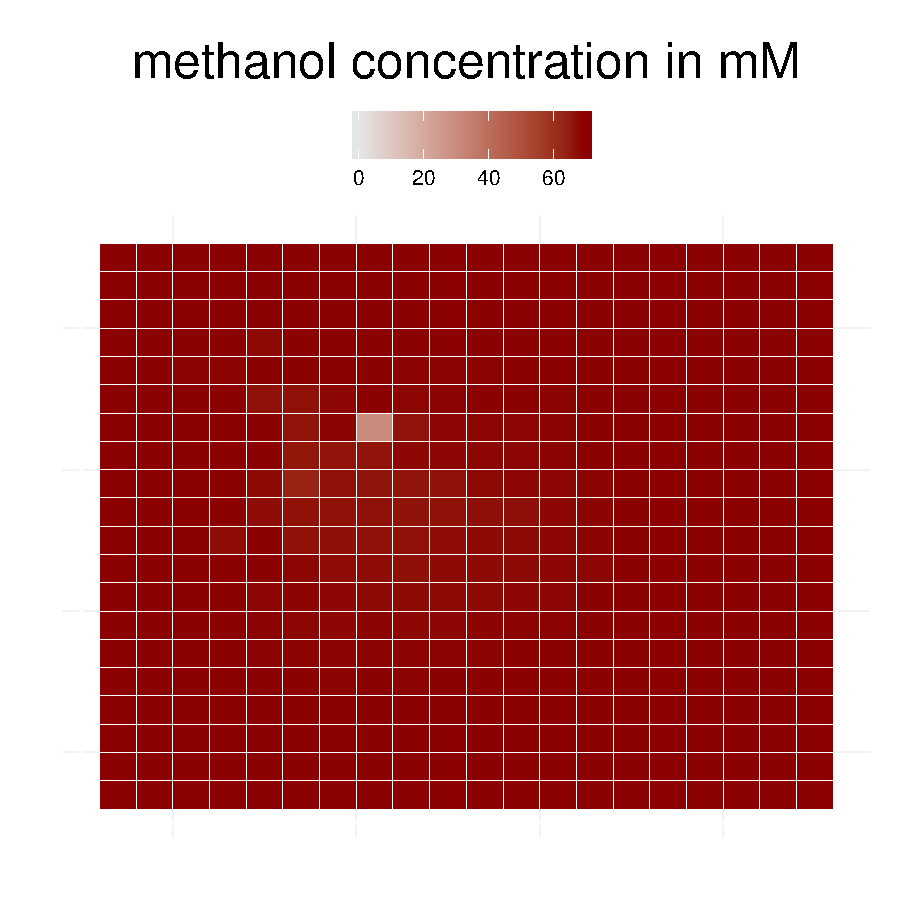
\includegraphics[width=\textwidth]{../results/img/barkeri_20x20_seed9659_methanol10a.pdf}
  \end{minipage}
  \begin{minipage}[t]{0.3\textwidth}
    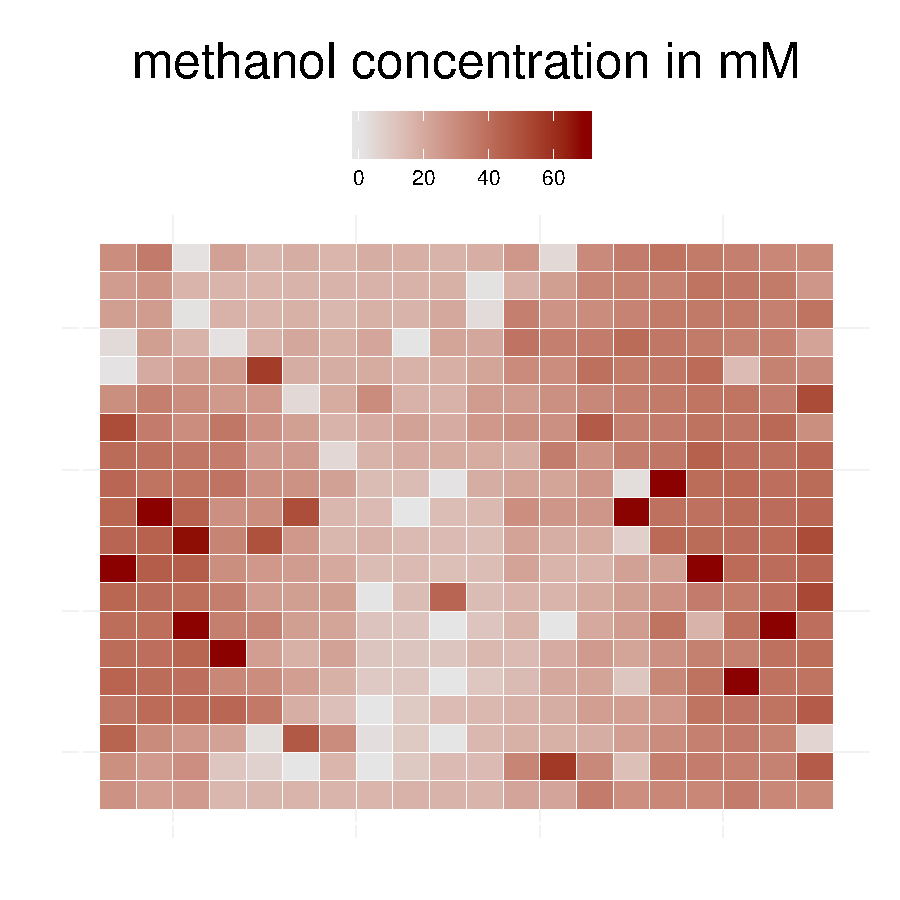
\includegraphics[width=\textwidth]{../results/img/barkeri_20x20_seed9659_methanol75.pdf}
  \end{minipage}
  \begin{minipage}[t]{0.3\textwidth}
    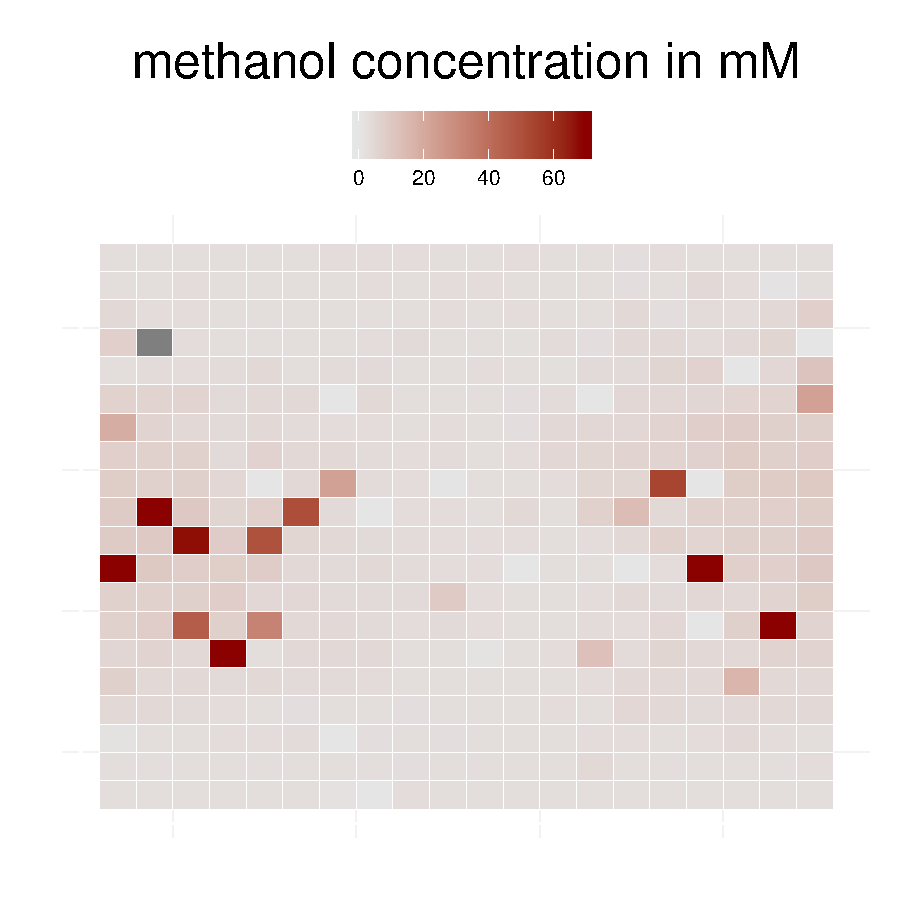
\includegraphics[width=\textwidth]{../results/img/barkeri_20x20_seed9659_methanol100a.pdf}
  \end{minipage}
  }
  \subfigure[]{
  \begin{minipage}[t]{0.3\textwidth}
    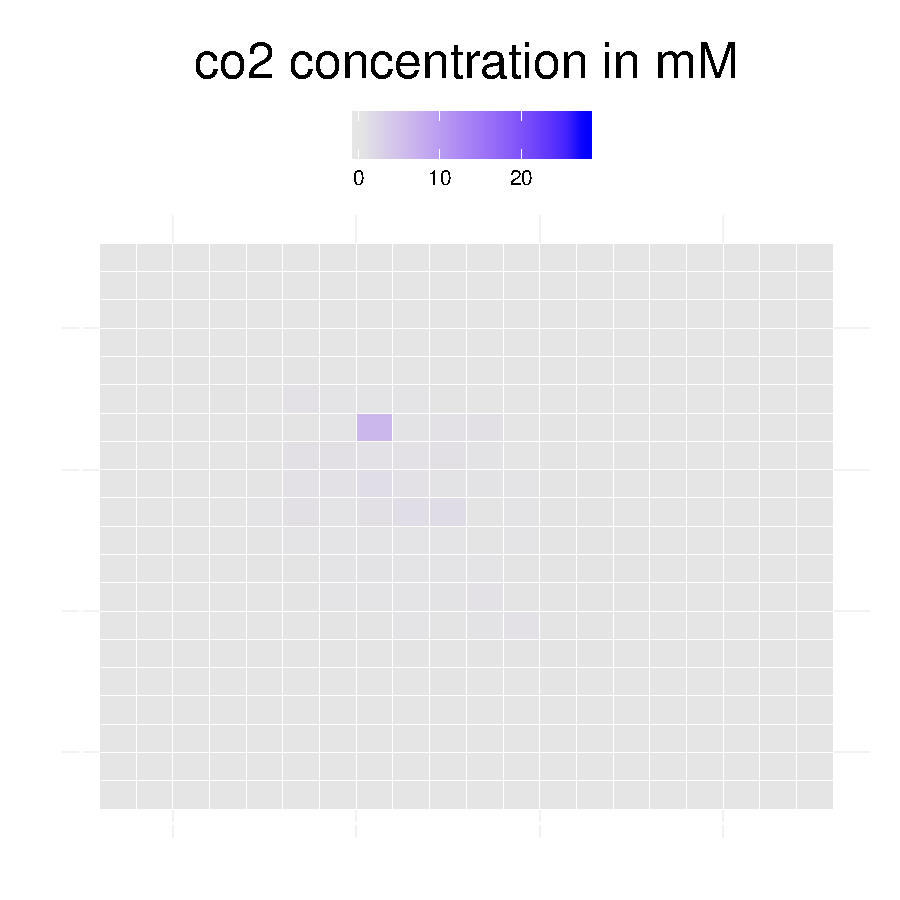
\includegraphics[width=\textwidth]{../results/img/barkeri_20x20_seed9659_co210a.pdf}
  \end{minipage}
  \begin{minipage}[t]{0.3\textwidth}
    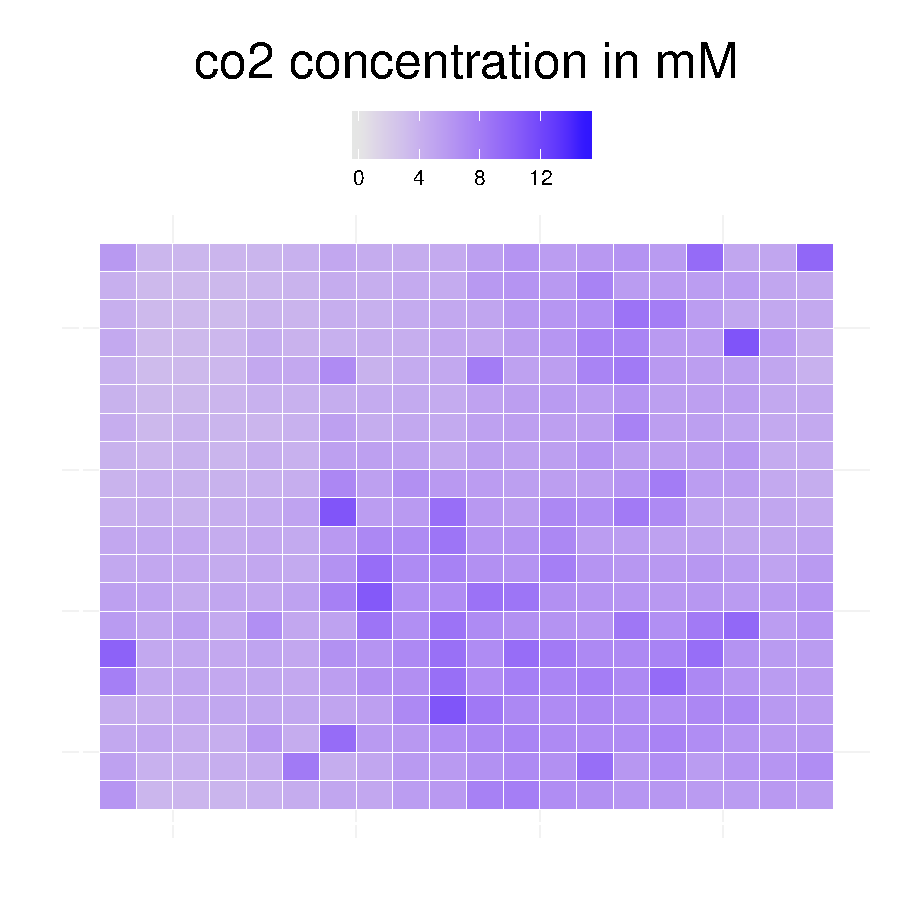
\includegraphics[width=\textwidth]{../results/img/barkeri_20x20_seed9659_co275.pdf}
  \end{minipage}
  \begin{minipage}[t]{0.3\textwidth}
    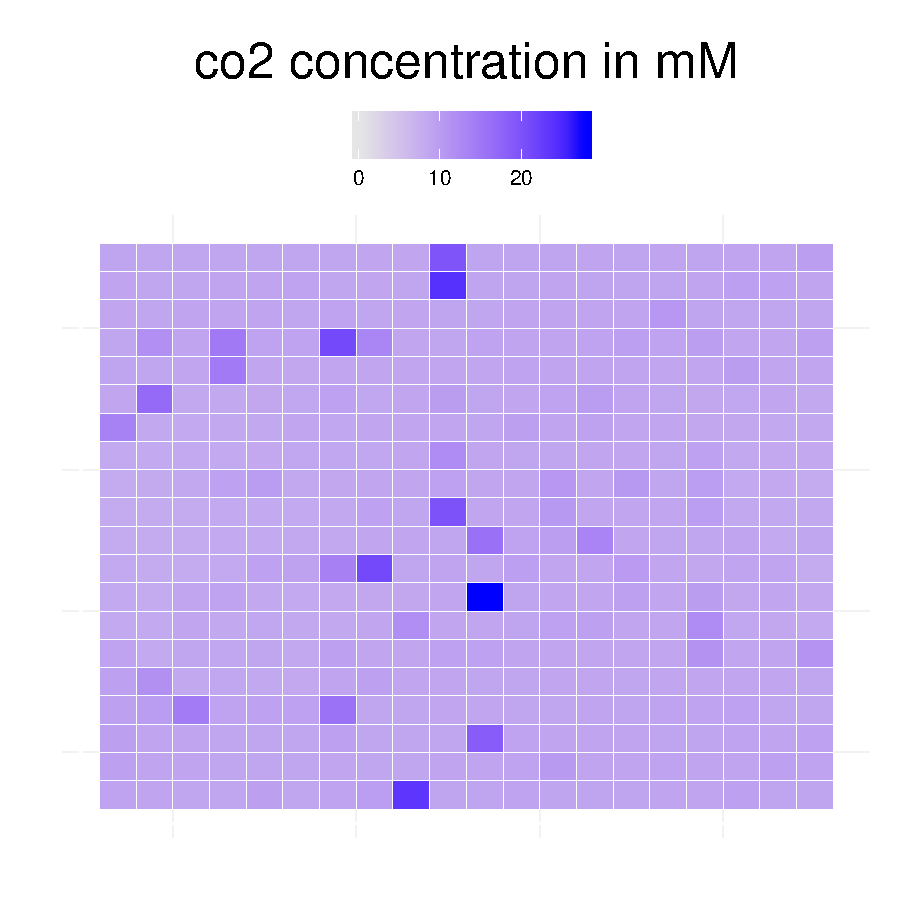
\includegraphics[width=\textwidth]{../results/img/barkeri_20x20_seed9659_co2100a.pdf}
  \end{minipage}
  }
  \subfigure[]{
  \begin{minipage}[t]{0.3\textwidth}
    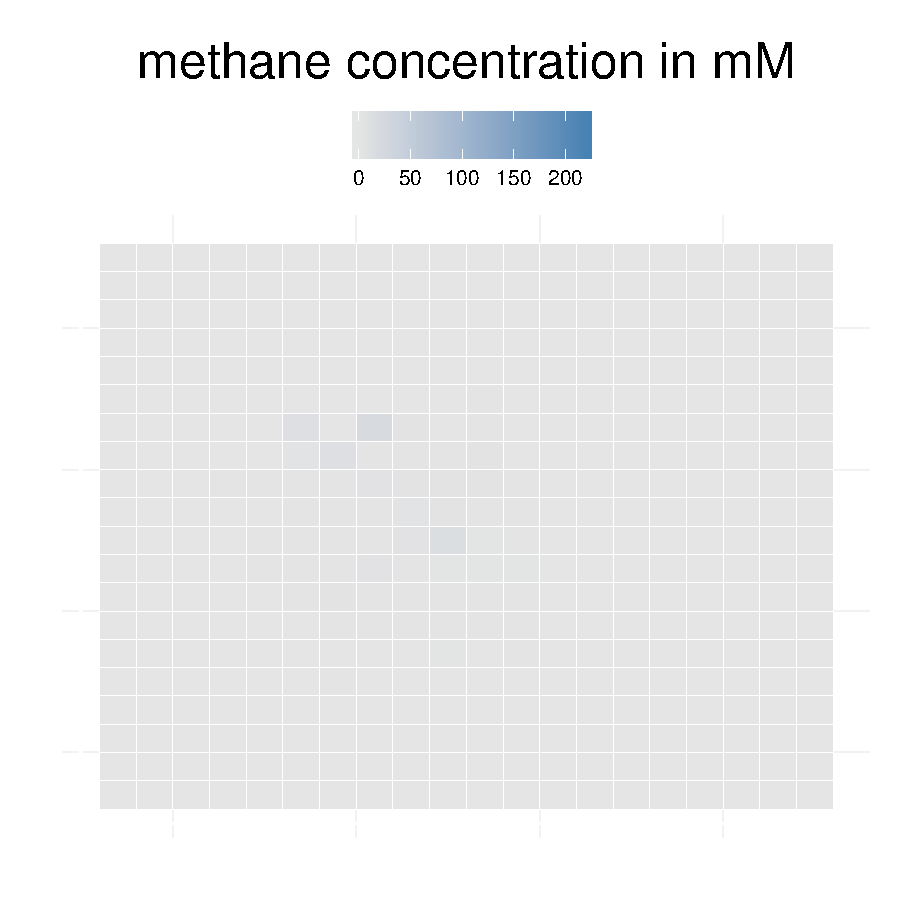
\includegraphics[width=\textwidth]{../results/img/barkeri_20x20_seed9659_meth10a.pdf}
  \end{minipage}
  \begin{minipage}[t]{0.3\textwidth}
    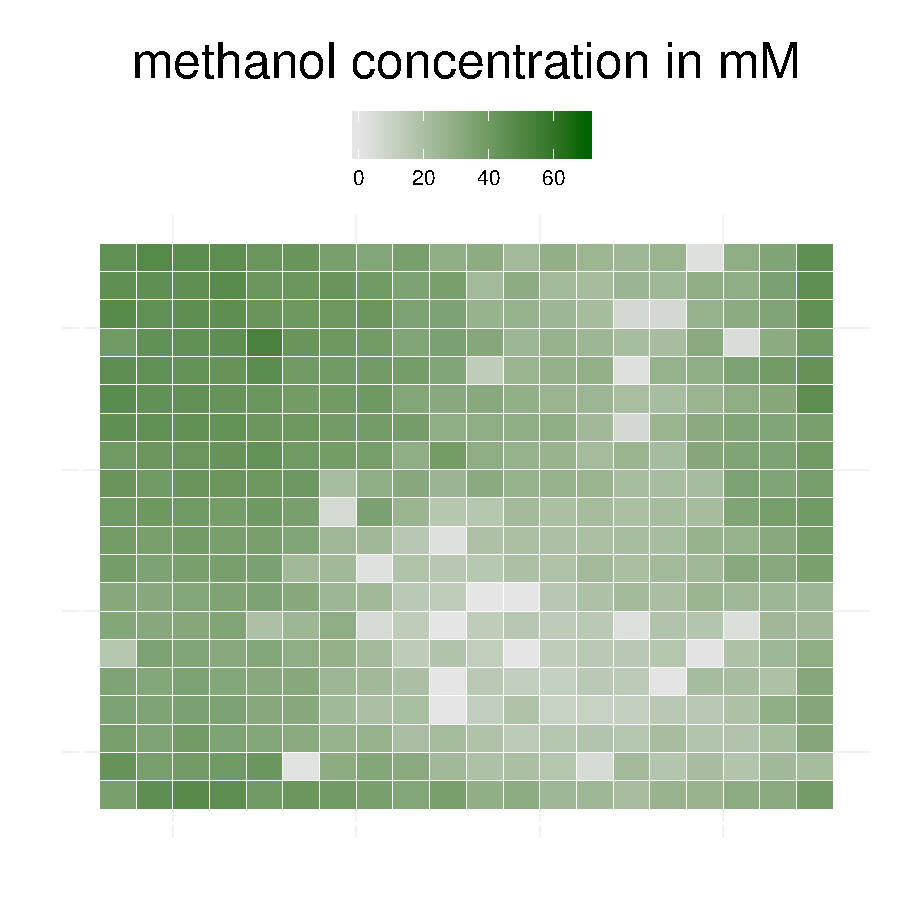
\includegraphics[width=\textwidth]{../results/img/barkeri_20x20_seed9659_meth75.pdf}
  \end{minipage}
  \begin{minipage}[t]{0.3\textwidth}
    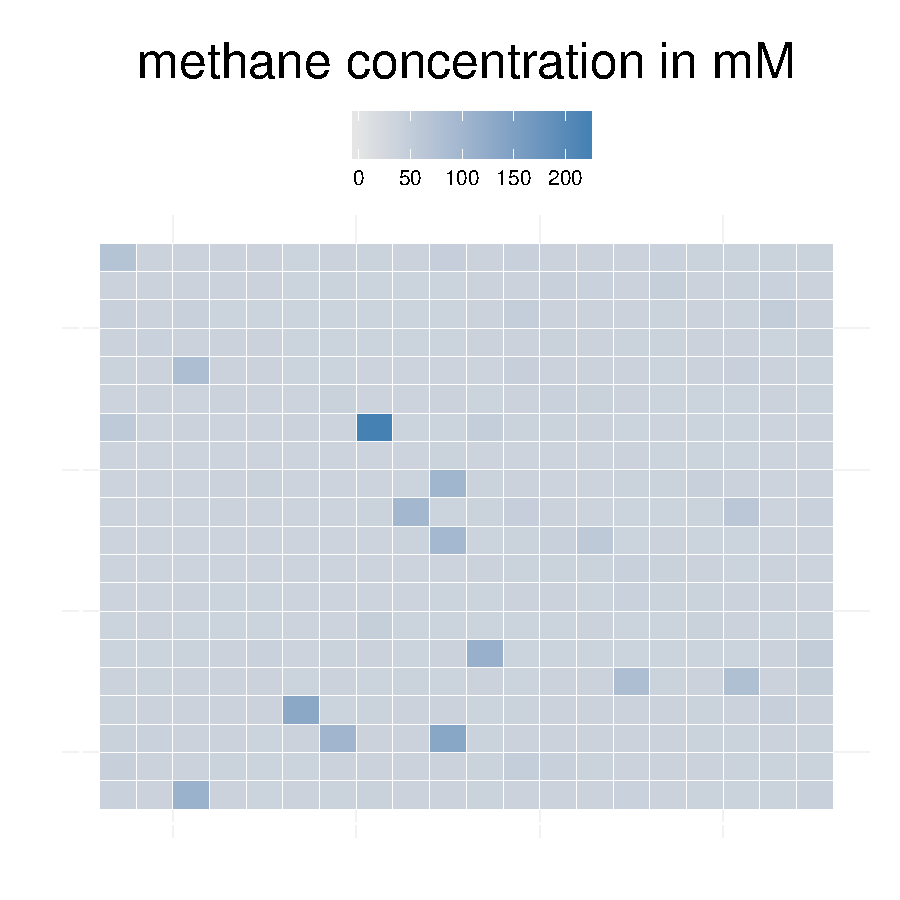
\includegraphics[width=\textwidth]{../results/img/barkeri_20x20_seed9659_meth100a.pdf}
  \end{minipage}
  }
  \caption{Population dynamics of the \emph{M. barkeri} model on a $20\times20$ grid, with bacterial movement (A) and concentrations of methanol (B), CO$_2$ (C) and methane (D) (of time step 10, 75 and 100). The seed of the random number generator was set to 9659.}
  %\caption{Population and metabolite dynamics of the \emph{M. barkeri} model on a $20\times20$ grid.}
  \label{fig:barkerigrids}
\end{figure}


\subsubsection{\textit{Clostridium beijerinckii}}
The \textit{C. beijerinckii} model was subjected to initial concentrations of glucose as a substrate, to generate a population model and monitor the production/consumption of various metabolites (Figure \hyperref[fig:beijersg]{\ref{fig:beijersg}}). In the first time steps glucose was consumed and hydrogen, C0$_2$, acetate, butyrate and succinate were produced in descending amounts. 
Compared to the other products hydrogen and CO$_2$ were produced much more.
The doubling time in the exponential phase was estimated as 6 iteration (h).
The population growth reached the stationary phase in approximately 45 iterations (h), after glucose was almost consumed. In the subsequent death phase no metabolites were produced or consumed. The population died out after 65 iterations.
According the dispersion of the microbes on the grid environment, substrates were consumed and metabolites produced (Figure \hyperref[fig:beijergrids]{\ref{fig:beijergrids}}).
\begin{figure}[h!]
  \centering
    \includegraphics[scale=0.45]{../results/img/beijerinckii_20x20_seed943_growth.pdf}
    \includegraphics[scale=0.45]{../results/img/beijerinckii_20x20_seed943_subs.pdf}
  \caption{Population dynamics of the \emph{C. beijerinckii} model on a $20\times20$ grid, with bacterial growth (A) and consumption/production of various metabolites (B). An initial concentration of 70\;mmol per grid cell of glucose was added to the environment. The seed of the random number generator was set to 943.}
  \label{fig:beijersg}
\end{figure}
\begin{figure}[h!]
  \centering
  \subfigure[]{
    \begin{minipage}[t]{0.3\textwidth}
    \includegraphics[width=\textwidth]{../results/img/beijerinckii_20x20_seed943_bac10.pdf}
  \end{minipage}
  \begin{minipage}[t]{0.3\textwidth}
    \includegraphics[width=\textwidth]{../results/img/beijerinckii_20x20_seed943_bac30.pdf}
  \end{minipage}
  \begin{minipage}[t]{0.3\textwidth}
    \includegraphics[width=\textwidth]{../results/img/beijerinckii_20x20_seed943_bac50.pdf}
  \end{minipage}
  }
  \subfigure[]{
  \begin{minipage}[t]{0.3\textwidth}
    \includegraphics[width=\textwidth]{../results/img/beijerinckii_20x20_seed943_glc20.pdf}
  \end{minipage}
  \begin{minipage}[t]{0.3\textwidth}
    \includegraphics[width=\textwidth]{../results/img/beijerinckii_20x20_seed943_glc40.pdf}
  \end{minipage}
  \begin{minipage}[t]{0.3\textwidth}
    \includegraphics[width=\textwidth]{../results/img/beijerinckii_20x20_seed943_glc50.pdf}
  \end{minipage}
  }
  \subfigure[]{
  \begin{minipage}[t]{0.3\textwidth}
    \includegraphics[width=\textwidth]{../results/img/beijerinckii_20x20_seed943_h220.pdf}
  \end{minipage}
  \begin{minipage}[t]{0.3\textwidth}
    \includegraphics[width=\textwidth]{../results/img/beijerinckii_20x20_seed943_h240.pdf}
  \end{minipage}
  \begin{minipage}[t]{0.3\textwidth}
    \includegraphics[width=\textwidth]{../results/img/beijerinckii_20x20_seed943_h250.pdf}
  \end{minipage}
  }
  \subfigure[]{
  \begin{minipage}[t]{0.3\textwidth}
    \includegraphics[width=\textwidth]{../results/img/beijerinckii_20x20_seed943_co220.pdf}
  \end{minipage}
  \begin{minipage}[t]{0.3\textwidth}
    \includegraphics[width=\textwidth]{../results/img/beijerinckii_20x20_seed943_co240.pdf}
  \end{minipage}
  \begin{minipage}[t]{0.3\textwidth}
    \includegraphics[width=\textwidth]{../results/img/beijerinckii_20x20_seed943_co250.pdf}
  \end{minipage}
  }
  \caption{Population dynamics of the \emph{C. beijerinckii} model on a $20\times20$ grid, with bacterial movement (A) and concentrations of glucose (B), hydrogen (C) and CO$_2$ (D) (of time step 20, 40 and 50). The seed of the random number generator was set to 943.}
   %\caption{Population and metabolite dynamics of the \emph{C. beijerinckii} model on a $20\times20$ grid.}
  \label{fig:beijergrids}
\end{figure}

\subsection{Mixed communities}
%To study the metabolic interactions of multiple species the individual models described in the previous sections were loaded in the same grid environment.
\subsubsection{\textit{Escherichia coli big} \& \textit{Methanosarcina barkeri}}
The joint simulation of the \textit{E. coli} and \textit{M. barkeri} was subjected to initial concentrations of glucose as a substrate for \textit{E. coli} and methanol as a substrate for \textit{M. barkeri}. In the first time steps the respective substrates were consumed and CO$_2$, acetate, ethanol, formate, water and methane were produced (Figure \hyperref[fig:besg]{\ref{fig:besg}}). Acetate was produced as a fermentation product of \textit{E. coli} and consumed by \textit{M. barkeri}. CO$_2$ was produced by \textit{E. coli} and \textit{M. barkeri}. \textit{E. coli} reached the stationary phase in iteration 90.
Since grid space was additionally occupied by \textit{M. barkeri}, the \textit{E. coli} population slightly grew after stationary phase of \textit{M. barkeri} in iteration 125. Both populations died out after iteration 175.
The doubling time in the exponential phase was estimated as 17 iterations (h) for \textit{E. coli} and 12 iterations (h) for \textit{M. barkeri}.
According the dispersion of the microbes on the grid environment, substrates were consumed and metabolites produced (Figure \hyperref[fig:cegrid]{\ref{fig:cegrid}}). The production of methane was found in grid positions occupied by \textit{M. barkeri} and glucose consumption was found in position occupied by \textit{E. coli}. In the later stages of growth acetate was consumed by \textit{M. barkeri}.
\begin{figure}[h!]
  \centering
    \includegraphics[scale=0.45]{../results/img/barkeri_ecoli_20x20_seed4612_growth.pdf}
    \includegraphics[scale=0.45]{../results/img/barkeri_ecoli_20x20_seed4612_subs.pdf}
  \caption{Population dynamics of the joint big \emph{E. coli} and \emph{M. barkeri} model on a $20\times20$ grid, with bacterial growth (A) and consumption/production of various metabolites (B). An initial concentration of 70\;mmol per grid cell of glucose and methanol was added to the environment. The seed of the random number generator was set to 4612.}
  \label{fig:besg}
\end{figure}
\begin{figure}[h!]
  \centering
  \subfigure[]{
    \begin{minipage}[t]{0.3\textwidth}
    \includegraphics[width=\textwidth]{../results/img/barkeri_ecoli_20x20_seed4612_bac50.pdf}
  \end{minipage}
  \begin{minipage}[t]{0.3\textwidth}
    \includegraphics[width=\textwidth]{../results/img/barkeri_ecoli_20x20_seed4612_bac100.pdf}
  \end{minipage}
  \begin{minipage}[t]{0.3\textwidth}
    \includegraphics[width=\textwidth]{../results/img/barkeri_ecoli_20x20_seed4612_bac150.pdf}
  \end{minipage}
  }
  \subfigure[]{
  \begin{minipage}[t]{0.3\textwidth}
    \includegraphics[width=\textwidth]{../results/img/barkeri_ecoli_20x20_seed4612_glc80.pdf}
  \end{minipage}
  \begin{minipage}[t]{0.3\textwidth}
    \includegraphics[width=\textwidth]{../results/img/barkeri_ecoli_20x20_seed4612_glc100a.pdf}
  \end{minipage}
  \begin{minipage}[t]{0.3\textwidth}
    \includegraphics[width=\textwidth]{../results/img/barkeri_ecoli_20x20_seed4612_glc130.pdf}
  \end{minipage}
  }
  \subfigure[]{
  \begin{minipage}[t]{0.3\textwidth}
    \includegraphics[width=\textwidth]{../results/img/barkeri_ecoli_20x20_seed4612_ace80.pdf}
  \end{minipage}
  \begin{minipage}[t]{0.3\textwidth}
    \includegraphics[width=\textwidth]{../results/img/barkeri_ecoli_20x20_seed4612_ace100a.pdf}
  \end{minipage}
  \begin{minipage}[t]{0.3\textwidth}
    \includegraphics[width=\textwidth]{../results/img/barkeri_ecoli_20x20_seed4612_ace130.pdf}
  \end{minipage}
  }
  \subfigure[]{
  \begin{minipage}[t]{0.3\textwidth}
    \includegraphics[width=\textwidth]{../results/img/barkeri_ecoli_20x20_seed4612_meth80.pdf}
  \end{minipage}
  \begin{minipage}[t]{0.3\textwidth}
    \includegraphics[width=\textwidth]{../results/img/barkeri_ecoli_20x20_seed4612_meth100a.pdf}
  \end{minipage}
  \begin{minipage}[t]{0.3\textwidth}
    \includegraphics[width=\textwidth]{../results/img/barkeri_ecoli_20x20_seed4612_meth130.pdf}
  \end{minipage}
  }
  \caption{Population dynamics of the joint big \emph{E. coli} and \emph{M. barkeri} model on a $20\times20$ grid, with bacterial movement (A) and concentrations of glucose (B), acetate (C) and methane (D) (of time step 80, 100 and 130). The seed of the random number generator was set to 4612.}
%  \caption{Population and metabolite dynamics of the joint \emph{E. coli} and \emph{M. barkeri} model.}
  \label{fig:begrid}
\end{figure}

\subsubsection{\textit{Escherichia coli big} \& \textit{Clostridium beijerinckii}}
The joint simulation of the \textit{E. coli} and \textit{C. beijerinckii} was subjected to initial concentrations of glucose as a substrate for both organisms. In the first time steps the substrate was competitively consumed by both species and CO$_2$, acetate, ethanol, butyrate, succinate and hydrogen was produced (Figure \hyperref[fig:cesg]{\ref{fig:cesg}}). In comparison to the other metabolites hydrogen and CO$_2$ had the highest concentrations at the end of the simulation.
Hydrogen, CO$_2$, butyrate and succinate were exclusively produced by \textit{C. beijerinckii}, whereas ethanol was produced by \textit{E. coli}. 
Acetate was produced by both species. \textit{C. beijerinckii} reached the stationary phase at 55 iterations and \textit{E. coli} at 60 iterations. Both organisms died at iteration 80. In the exponential phase \textit{C. beijerinckii} had an approximate duplication time of 8 iterations and \textit{E. coli} of 11 iterations.

According the dispersion of the microbes on the grid environment, substrates were consumed and metabolites produced (Figure \hyperref[fig:cegrid]{\ref{fig:cegrid}}). Hydrogen production was found in \textit{C. beijerinckii} occupied grid positions and ethanol production in \textit{E. coli} occupied positions.
\begin{figure}[h!]
  \centering
    \includegraphics[scale=0.45]{../results/img/ecoli_beijerinckii_20x20_seed5147_growth.pdf}
    \includegraphics[scale=0.45]{../results/img/ecoli_beijerinckii_20x20_seed5147_subs.pdf}
  \caption{Population dynamics of the joint big \emph{E. coli} and \emph{C. beijerinckii} model on a $20\times20$ grid, with bacterial growth (A) and consumption/production of various metabolites (B). An initial concentration of 70\;mmol per grid cell of glucose was added to the environment. The seed of the random number generator was set to 5147.}
  \label{fig:cesg}
\end{figure}
\begin{figure}[h!]
  \centering
  \subfigure[]{
    \begin{minipage}[t]{0.3\textwidth}
    \includegraphics[width=\textwidth]{../results/img/ecoli_beijerinckii_20x20_seed5147_bac25.pdf}
  \end{minipage}
  \begin{minipage}[t]{0.3\textwidth}
    \includegraphics[width=\textwidth]{../results/img/ecoli_beijerinckii_20x20_seed5147_bac55.pdf}
  \end{minipage}
  \begin{minipage}[t]{0.3\textwidth}
    \includegraphics[width=\textwidth]{../results/img/ecoli_beijerinckii_20x20_seed5147_bac65.pdf}
  \end{minipage}
  }
  \subfigure[]{
  \begin{minipage}[t]{0.3\textwidth}
    \includegraphics[width=\textwidth]{../results/img/ecoli_beijerinckii_20x20_seed5147_glc25.pdf}
  \end{minipage}
  \begin{minipage}[t]{0.3\textwidth}
    \includegraphics[width=\textwidth]{../results/img/ecoli_beijerinckii_20x20_seed5147_glc55.pdf}
  \end{minipage}
  \begin{minipage}[t]{0.3\textwidth}
    \includegraphics[width=\textwidth]{../results/img/ecoli_beijerinckii_20x20_seed5147_glc65.pdf}
  \end{minipage}
  }
  \subfigure[]{
  \begin{minipage}[t]{0.3\textwidth}
    \includegraphics[width=\textwidth]{../results/img/ecoli_beijerinckii_20x20_seed5147_h225.pdf}
  \end{minipage}
  \begin{minipage}[t]{0.3\textwidth}
    \includegraphics[width=\textwidth]{../results/img/ecoli_beijerinckii_20x20_seed5147_h255.pdf}
  \end{minipage}
  \begin{minipage}[t]{0.3\textwidth}
    \includegraphics[width=\textwidth]{../results/img/ecoli_beijerinckii_20x20_seed5147_h265.pdf}
  \end{minipage}
  }
  \subfigure[]{
  \begin{minipage}[t]{0.3\textwidth}
    \includegraphics[width=\textwidth]{../results/img/ecoli_beijerinckii_20x20_seed5147_eth25.pdf}
  \end{minipage}
  \begin{minipage}[t]{0.3\textwidth}
    \includegraphics[width=\textwidth]{../results/img/ecoli_beijerinckii_20x20_seed5147_eth55.pdf}
  \end{minipage}
  \begin{minipage}[t]{0.3\textwidth}
    \includegraphics[width=\textwidth]{../results/img/ecoli_beijerinckii_20x20_seed5147_eth65.pdf}
  \end{minipage}
  }
  \caption{Population dynamics of the joint big \emph{E. coli} and \emph{C. beijerinckii} model on a $20\times20$ grid, with bacterial movement (A) and concentrations of glucose (B), hydrogen (C) and ethanol (D) (of time step 25, 55 and 65). The seed of the random number generator was set to 5147.}
  %\caption{Dynamics of the joint \emph{E. coli} and \emph{C. beijerinckii} model on a $20\times20$ grid.}
  \label{fig:cegrid}
\end{figure}

\subsubsection{\textit{Clostridium beijerinckii} \& \textit{Methanosarcina barkeri}}
The joint simulation of the \textit{M. barkeri} and \textit{C. beijerinckii} was subjected to initial concentrations of glucose as a exclusive substrate for \textit{C. beijerinckii}. In the first time steps the substrate was consumed by \textit{C. beijerinckii} and CO$_2$, hydrogen, acetate, butyrate and succinate was produced (Figure \hyperref[fig:cbsg]{\ref{fig:cbsg}}). 
In comparison to the other metabolites hydrogen and CO$_2$ had the highest concentrations at the stationary phase of \textit{C. beijerinckii} reached at approximately 60 iterations. The population of \textit{C. beijerinckii} died out at iteration 80 and \textit{M. barkeri} started growing exponentially by taking the produced hydrogen and CO$_2$ as substrates. 
In the later phases of growth the produced acetate was used as a substrate. The stationary phase of \textit{M. barkeri} was reached at iteration 170. 
During growth \textit{M. barkeri} produced methane and water by consuming CO$_2$ and almost the total hydrogen produced by \textit{C. beijerinckii}. 
In the exponential phase \textit{C. beijerinckii} had an approximate duplication time of 8 iterations and \textit{M. barkeri} of 12 iterations.
According the dispersion of the microbes on the grid environment, substrates were consumed and metabolites produced (Figure \hyperref[fig:cbgrid]{\ref{fig:cbgrid}}). Hydrogen production was found in \textit{C. beijerinckii} occupied grid positions and methane production in \textit{M. barkeri} occupied positions.
\begin{figure}[h!]
  \centering
    \includegraphics[scale=0.45]{../results/img/barkeri_beijerinckii_20x20_seed6764_growth.pdf}
    \includegraphics[scale=0.45]{../results/img/barkeri_beijerinckii_20x20_seed6764_subs.pdf}
  \caption{Population dynamics of the joint \emph{M. barkeri} and \emph{C. beijerinckii} model on a $20\times20$ grid, with bacterial growth (A) and consumption/production of various metabolites (B). An initial concentration of 70\;mmol per grid cell of glucose was added to the environment. The seed of the random number generator was set to 6764.}
  \label{fig:cbsg}
\end{figure}
\begin{figure}[h!]
  \centering
  \subfigure[]{
    \begin{minipage}[t]{0.3\textwidth}
    \includegraphics[width=\textwidth]{../results/img/barkeri_beijerinckii_20x20_seed6764_bac50.pdf}
  \end{minipage}
  \begin{minipage}[t]{0.3\textwidth}
    \includegraphics[width=\textwidth]{../results/img/barkeri_beijerinckii_20x20_seed6764_bac100.pdf}
  \end{minipage}
  \begin{minipage}[t]{0.3\textwidth}
    \includegraphics[width=\textwidth]{../results/img/barkeri_beijerinckii_20x20_seed6764_bac150.pdf}
  \end{minipage}
  }
  \subfigure[]{
  \begin{minipage}[t]{0.3\textwidth}
    \includegraphics[width=\textwidth]{../results/img/barkeri_beijerinckii_20x20_seed6764_glc50.pdf}
  \end{minipage}
  \begin{minipage}[t]{0.3\textwidth}
    \includegraphics[width=\textwidth]{../results/img/barkeri_beijerinckii_20x20_seed6764_glc100.pdf}
  \end{minipage}
  \begin{minipage}[t]{0.3\textwidth}
    \includegraphics[width=\textwidth]{../results/img/barkeri_beijerinckii_20x20_seed6764_glc150.pdf}
  \end{minipage}
  }
  \subfigure[]{
  \begin{minipage}[t]{0.3\textwidth}
    \includegraphics[width=\textwidth]{../results/img/barkeri_beijerinckii_20x20_seed6764_h250a.pdf}
  \end{minipage}
  \begin{minipage}[t]{0.3\textwidth}
    \includegraphics[width=\textwidth]{../results/img/barkeri_beijerinckii_20x20_seed6764_h2100a.pdf}
  \end{minipage}
  \begin{minipage}[t]{0.3\textwidth}
    \includegraphics[width=\textwidth]{../results/img/barkeri_beijerinckii_20x20_seed6764_h2150a.pdf}
  \end{minipage}
  }
  \subfigure[]{
  \begin{minipage}[t]{0.3\textwidth}
    \includegraphics[width=\textwidth]{../results/img/barkeri_beijerinckii_20x20_seed6764_meth50a.pdf}
  \end{minipage}
  \begin{minipage}[t]{0.3\textwidth}
    \includegraphics[width=\textwidth]{../results/img/barkeri_beijerinckii_20x20_seed6764_meth100a.pdf}
  \end{minipage}
  \begin{minipage}[t]{0.3\textwidth}
    \includegraphics[width=\textwidth]{../results/img/barkeri_beijerinckii_20x20_seed6764_meth150a.pdf}
  \end{minipage}
  }
  \caption{Dynamics of the joint \emph{M. barkeri} and \emph{C. beijerinckii} model on a $20\times20$ grid, with bacterial movement (A) and concentrations of glucose (B), hydrogen (C) and methanol (D) (time step 50, 100 and 150). The seed of the random number generator was set to 6764.}
  \label{fig:cbgrid}
  %\caption{Dynamics of the joint \emph{M. barkeri} and \emph{C. beijerinckii} model on a $20\times20$ grid.}
\end{figure}

%\subsection{Spatial and time-wise heterogeneity}
%\subsubsection{Substrate gradients}
%\subsubsection{Delayed bacterial input}
